% Options for packages loaded elsewhere
\PassOptionsToPackage{unicode}{hyperref}
\PassOptionsToPackage{hyphens}{url}
%
\documentclass[
]{article}
\usepackage{amsmath,amssymb}
\usepackage{iftex}
\ifPDFTeX
  \usepackage[T1]{fontenc}
  \usepackage[utf8]{inputenc}
  \usepackage{textcomp} % provide euro and other symbols
\else % if luatex or xetex
  \usepackage{unicode-math} % this also loads fontspec
  \defaultfontfeatures{Scale=MatchLowercase}
  \defaultfontfeatures[\rmfamily]{Ligatures=TeX,Scale=1}
\fi
\usepackage{lmodern}
\ifPDFTeX\else
  % xetex/luatex font selection
\fi
% Use upquote if available, for straight quotes in verbatim environments
\IfFileExists{upquote.sty}{\usepackage{upquote}}{}
\IfFileExists{microtype.sty}{% use microtype if available
  \usepackage[]{microtype}
  \UseMicrotypeSet[protrusion]{basicmath} % disable protrusion for tt fonts
}{}
\makeatletter
\@ifundefined{KOMAClassName}{% if non-KOMA class
  \IfFileExists{parskip.sty}{%
    \usepackage{parskip}
  }{% else
    \setlength{\parindent}{0pt}
    \setlength{\parskip}{6pt plus 2pt minus 1pt}}
}{% if KOMA class
  \KOMAoptions{parskip=half}}
\makeatother
\usepackage{xcolor}
\usepackage[margin=1in]{geometry}
\usepackage{graphicx}
\makeatletter
\def\maxwidth{\ifdim\Gin@nat@width>\linewidth\linewidth\else\Gin@nat@width\fi}
\def\maxheight{\ifdim\Gin@nat@height>\textheight\textheight\else\Gin@nat@height\fi}
\makeatother
% Scale images if necessary, so that they will not overflow the page
% margins by default, and it is still possible to overwrite the defaults
% using explicit options in \includegraphics[width, height, ...]{}
\setkeys{Gin}{width=\maxwidth,height=\maxheight,keepaspectratio}
% Set default figure placement to htbp
\makeatletter
\def\fps@figure{htbp}
\makeatother
\setlength{\emergencystretch}{3em} % prevent overfull lines
\providecommand{\tightlist}{%
  \setlength{\itemsep}{0pt}\setlength{\parskip}{0pt}}
\setcounter{secnumdepth}{-\maxdimen} % remove section numbering
% definitions for citeproc citations
\NewDocumentCommand\citeproctext{}{}
\NewDocumentCommand\citeproc{mm}{%
  \begingroup\def\citeproctext{#2}\cite{#1}\endgroup}
\makeatletter
 % allow citations to break across lines
 \let\@cite@ofmt\@firstofone
 % avoid brackets around text for \cite:
 \def\@biblabel#1{}
 \def\@cite#1#2{{#1\if@tempswa , #2\fi}}
\makeatother
\newlength{\cslhangindent}
\setlength{\cslhangindent}{1.5em}
\newlength{\csllabelwidth}
\setlength{\csllabelwidth}{3em}
\newenvironment{CSLReferences}[2] % #1 hanging-indent, #2 entry-spacing
 {\begin{list}{}{%
  \setlength{\itemindent}{0pt}
  \setlength{\leftmargin}{0pt}
  \setlength{\parsep}{0pt}
  % turn on hanging indent if param 1 is 1
  \ifodd #1
   \setlength{\leftmargin}{\cslhangindent}
   \setlength{\itemindent}{-1\cslhangindent}
  \fi
  % set entry spacing
  \setlength{\itemsep}{#2\baselineskip}}}
 {\end{list}}
\usepackage{calc}
\newcommand{\CSLBlock}[1]{\hfill\break\parbox[t]{\linewidth}{\strut\ignorespaces#1\strut}}
\newcommand{\CSLLeftMargin}[1]{\parbox[t]{\csllabelwidth}{\strut#1\strut}}
\newcommand{\CSLRightInline}[1]{\parbox[t]{\linewidth - \csllabelwidth}{\strut#1\strut}}
\newcommand{\CSLIndent}[1]{\hspace{\cslhangindent}#1}
\usepackage{titling}
\usepackage{booktabs}
\usepackage{pdflscape}
\usepackage{pgfplots}
\usepackage{tikz}
\usetikzlibrary{positioning, arrows, shapes.geometric}
\usepackage[dvipsnames, table]{xcolor}
\usepackage{lscape}
\usepackage{float}
\usepackage{amsmath}
\usepackage{fancyhdr}
\usepackage{caption}
\captionsetup[figure]{labelformat=empty}
\captionsetup[table]{labelformat=empty}
\usepackage{etoolbox}
\fancyhf{}
\rfoot{\thepage}
\pagenumbering{gobble}
\pretitle{\begin{center}\LARGE}
\posttitle{\par\end{center}}
\preauthor{\begin{center}\large}
\postauthor{\par\end{center}}
\predate{\begin{center}\small}
\postdate{\par\medskip
Department of Criminology, School of Social Sciences, The University of Manchester\\
\textbf{CRIM30610 Long Dissertation}\\
\textbf{Supervisor:} Thiago R. Oliveira\\
\textbf{Word count:} 8418/9000\\
\end{center}\newpage
\pagenumbering{arabic}
}
\usepackage{booktabs}
\usepackage{longtable}
\usepackage{array}
\usepackage{multirow}
\usepackage{wrapfig}
\usepackage{float}
\usepackage{colortbl}
\usepackage{pdflscape}
\usepackage{tabu}
\usepackage{threeparttable}
\usepackage{threeparttablex}
\usepackage[normalem]{ulem}
\usepackage{makecell}
\usepackage{xcolor}
\usepackage{tabularray}
\usepackage[normalem]{ulem}
\usepackage{graphicx}
\usepackage{rotating}
\UseTblrLibrary{booktabs}
\UseTblrLibrary{siunitx}
\NewTableCommand{\tinytableDefineColor}[3]{\definecolor{#1}{#2}{#3}}
\newcommand{\tinytableTabularrayUnderline}[1]{\underline{#1}}
\newcommand{\tinytableTabularrayStrikeout}[1]{\sout{#1}}
\ifLuaTeX
  \usepackage{selnolig}  % disable illegal ligatures
\fi
\usepackage{bookmark}
\IfFileExists{xurl.sty}{\usepackage{xurl}}{} % add URL line breaks if available
\urlstyle{same}
\hypersetup{
  pdftitle={Undergraduate Dissertation: Cold Calculations - How Conflict Characteristics Shape External Support in Armed Conflicts},
  pdfauthor={Student ID: 11004503},
  hidelinks,
  pdfcreator={LaTeX via pandoc}}

\title{Undergraduate Dissertation: Cold Calculations - How Conflict
Characteristics Shape External Support in Armed Conflicts}
\author{Student ID: 11004503}
\date{08/05/2025}

\begin{document}
\maketitle

{
\setcounter{tocdepth}{2}
\tableofcontents
}
\newpage

\section{Table of Figures}\label{table-of-figures}

\begin{center}
\begin{tabular}{l l r}
\textbf{Type} & \textbf{Title} & \textbf{Page} \\

\\[-0.3em]
\multicolumn{3}{l}{\textbf{Tables}} \\[0.3em]
Table 1 & Variables used in the analysis & 13 \\
Table 2 & Regression Results – External Support Determinants & 20 \\
Table 3 & Statistical Significance in the RE and FE Logistic Regression Models & 21 \\
Table 4 & RE and FE Logistic and PPML Regression Results & 24 \\[1.2em]

\multicolumn{3}{l}{\textbf{Figures}} \\[0.3em]
Figure 1 & Directed Acyclic Graph on Conflict Characteristics and External Support & 10 \\
Figure 2 & World armed conflicts by intensity level & 18 \\[0.3em]
Figure 3 & Mean and Median Conflict Duration by Region & 18 \\
Figure 4 & Direct and Indirect Support, 1975–2017 & 19 \\[1.2em]

\multicolumn{3}{l}{\textbf{Appendices}} \\[0.3em]
Appendix 1 & State-based Conflicts by Region, 1975–2017 & 26 \\
Appendix 2 & State-based Conflicts by Type of Conflict, 1975–2017 & 26 \\
Appendix 3 & Conflict Type by Region & 27 \\
Appendix 4 & Evolution of State-based Conflicts by Incompatibility, 1975–2017 & 27 \\
Appendix 5 & Evolution of External Support: Bilateral vs Coalition & 28 \\
Appendix 6 & Statistical Significance in the RE Linear Regression models & 29 \\

\end{tabular}
\end{center}

\newpage

\section{Declaration and Copyright
statement}\label{declaration-and-copyright-statement}

\subsection{Dissertation Declaration}\label{dissertation-declaration}

This work is all the author's original work unless referenced clearly to
the contrary. No portion of the work referred to in the dissertation has
been submitted in support of an application for another degree or
qualification of this or any other university or other institute of
learning.

\subsection{Dissertation Intellectual Property
Statement}\label{dissertation-intellectual-property-statement}

The author of this dissertation (including any appendices and/or
schedules to this dissertation) owns certain copyright or related rights
in it (the ``Copyright'') and she has given The University of Manchester
certain rights to use such Copyright, including for administrative
purposes.

\begin{enumerate}
\def\labelenumi{\roman{enumi}.}
\item
  Copies of this dissertation, either in full or in extracts and whether
  in hard or electronic copy, may be made only in accordance with the
  Copyright, Designs and Patents Act 1988 (as amended) and regulations
  issued under it or, where appropriate, in accordance with licensing
  agreements which the University has entered into. This page must form
  part of any such copies made.
\item
  The ownership of certain Copyright, patents, designs, trademarks and
  other intellectual property (the ``Intellectual Property'') and any
  reproductions of copyright works in the dissertation, for example
  graphs and tables (``Reproductions''), which may be described in this
  dissertation, may not be owned by the author and may be owned by third
  parties. Such Intellectual Property and Reproductions cannot and must
  not be made available for use without the prior written permission of
  the owner(s) of the relevant Intellectual Property and/or
  Reproductions.
\item
  Further information on the conditions under which disclosure,
  publication and commercialisation of this dissertation, the Copyright
  and any Intellectual Property and/or Reproductions described in it may
  take place is available in the University IP Policy, in any relevant
  Dissertation restriction declarations deposited in the University
  Library, and The University Library's regulations.
\end{enumerate}

\subsection{Data availability
statement}\label{data-availability-statement}

All analyses were conducted in R (R Core Team (2025)), with the analytic
code and input data made publicly available on
\href{https://github.com/celine-felicit/Dissertation-Code}{GitHub} to
ensure transparency and facilitate replication.

\section{Abstract}\label{abstract}

Despite its relevance to violence, victimisation, and state power,
Criminology has historically neglected the study of armed conflicts
(Hagan (2015); Jamieson (2003); Ruggiero (2015); McGarry and Walklate
(2015)). This dissertation aims to bridge this gap, using random and
fixed effects logistic regression to examine the impact of conflict
characteristics on the provision of external support. It seeks to
provide insights into the motives and strategies of external supporters,
essential for discussions around liability and responsibility in armed
conflicts. Aligning with existing literature, the findings of this study
suggest that external supporters tailor the provision of specific
indirect support to specific conflict dynamics (Schultz (2010); Bapat
(2012); Sawyer et al. (2015)). Based in criminological research on
violence (Collins (2008) in Rafter (2016)) this suggests a `cold',
calculated approach to the provision of external support, where external
supporters consider the conflict dynamics and the potential for
escalation before providing support. This research contributes to a more
comprehensive understanding of the interplay between external
interventions and conflict dynamics, bridging critical gaps in
criminology and offering a starting point for criminological discussion
around the liability and responsibility of external supporters.

\newpage

\section{Introduction}\label{introduction}

Despite a reduction in conflicts and deaths, the past decade remains the
most violent on record (Davies et al. (2024)). Today, although conflicts
are largely fought by developing nations, they rely heavily on advanced
military equipment produced by industrial countries, reinforcing
military over social investments (Sivard (1996)). The prevalence and
complexity of external support (ES) in armed conflicts (AC) have grown
significantly over the past decades. From 1975 to 2017, 80\% of
intrastate conflicts involved at least one instance of ES, with state
actors being the predominant supporters (Meier et al. (2023)). Recent
years have seen systemic shifts in ES, characterised by the rise of
multilateral coalitions and collaborative interventions. Nearly
one-third of all support instances now involve such coalitions,
emphasising burden-sharing and legitimacy (Meier et al. (2023)).
However, recent developments, such as the United States cutting off
significant amounts of its financial and military support for Ukraine,
and humanitarian aid to Syria (Sandefur and Kenny (2025); UN (2025)),
cast doubt on the future of military alliances and joint defence
initiatives like the North Atlantic Treaty Organisation (NATO), as well
as the accountability and durability of assistance. With many
geopolitical tensions and conflicts ongoing, discussions around AC and
ES are crucial to the political environment and international relations,
raising questions around the responsibility and accountability of
external supporters, especially when military actions turn into war
crimes.

While an extremely timely topic, Criminology has historically neglected
AC (Hagan (2015); Jamieson (2003); Ruggiero (2015); McGarry and Walklate
(2015)), let alone ES. But even in research on ES, the content of
interventions remains underexplored, despite its impact on conflict
trajectories (see for example Cunningham (2016); Karlén (2017); Aydin
and Regan (2012)). This research adopts an interdisciplinary approach,
integrating Criminology, Peace and Conflict Studies, and Economics to
examine whether conflict characteristics affect the provision of ES and
identify trends and conditions under which ES is provided. By
distinguishing between support types, it aims to provide a more robust
understanding of the role of external supporters and their motives,
essential for further discussions around liability and responsibility.
In doing so, it bridges critical gaps in Criminology, contributing to a
more comprehensive understanding of the interplay between external
interventions and conflict dynamics.

This dissertation addresses three research questions: (1) Do conflict
characteristics influence the provision of ES? (2) Do they affect the
form of support provided? (3) Does coalition-based support influence
what type of support is provided? The data comes from two Uppsala
Conflict Data Program (UCDP) datasets: the Dyadic Dataset (Version
18.1), covering conflict characteristics between 1946 and 2018 (Harbom
et al. (2008); Pettersson and Eck (2018)), and the External Support
Dataset (Version 18.1), which captures ten forms of ES between 1975 and
2017 (Meier et al. (2023)). Together, these sources provide a robust
foundation for quantitatively analysing the relationship between
conflict characteristics and ES. To answer the research questions, the
study uses fixed and random effects logistic regression models, allowing
for the examination of both within- and between-dyad variation. These
methods are well suited to the dyadic nature of AC data and support the
identification of strategic patterns in support provision---insights
essential for discussions on the liability and responsibility of
external actors. Therefore, this dissertation contributes to a more
nuanced understanding of the interplay between external interventions
and conflict dynamics, addressing critical gaps in criminological
literature on accountability in AC. The dissertation is structured as
follows: First, existing literature on AC and ES is reviewed,
highlighting gaps in criminological scholarship and introducing the
conceptual lens of `hot' versus `cold' mass violence. The research
design and theoretical framework are then described, followed by the
methodology, data, and operationalisation. Following the presentation of
the findings, it finishes with the discussion and concluding
reflections.

\section{Literature Review}\label{literature-review}

The landscape of AC has shifted in recent decades, with a rise in
internationalised intrastate conflicts where external states support
non-state actors opposing governments (Davies et al. (2024)). AC herein
is defined as `a contested incompatibility that concerns government
and/or territory where the use of armed force between two parties, of
which at least one is the government of a state, results in at least 25
battle-related deaths in a calendar year' (Themnér (2018), p.2). The
primary parties in such conflicts include governments, which control the
state capital, and opposition organisations, which are formally
organised groups using armed force to influence the outcome of the
incompatibility.

Although developing nations fight most of today's conflicts, they are
often fought with weapons from industrialised countries, reflecting
20th-century technological advancements (Sivard (1996)). As geopolitical
tensions rise, the role of ES in these conflicts has become a central
topic of discussion (Federle et al. (2024)). ES, defined as militarily
relevant assistance provided by outside parties to active conflicts, is
distinct from peacetime activities like arms trade or security reforms
(Meier et al. (2023); Meier (2022)). This support aims to enhance the
recipient's military capabilities and is provided with the clear intent
of facilitating military victory over the opposing side (Cunningham
(2010); Gregory (2000)). It includes materiel, knowledge, or services
directly aiding warfare but excludes unintentional support like
sanctions that weakens a conflict party but is not intended to support
the other side. Additionally, diplomatic efforts, humanitarian aid, and
mediation offers do not qualify as ES since they do not directly
contribute to the military outcome (Meier (2022)). The external nature
of support is determined by whether the provider is not a primary
warring party in the conflict, even if present in the same territory.

Foreign military operations, though a small portion of defence spending,
are pivotal in defining international relations and interventions (Marín
(2021)). Understanding why and how states intervene and the consequences
of different types of support is vital to analysing external
involvement. The interplay between conflict characteristics and ES is
complex, with interventions - whether direct military actions or
indirect aid - often prolonging hostilities and complicating peace
efforts (Sawyer et al. (2015); Karlén (2023); Regan (2002)). This
research seeks to explore these themes, examining how conflict
characteristics shape external interventions.

\subsection{The study of armed conflicts in
Criminology}\label{the-study-of-armed-conflicts-in-criminology}

Like many other social sciences, Criminology has historically neglected
AC, despite its relevance to violence, victimisation, and state power
(Hagan (2015); Jamieson (2003); Ruggiero (2015); McGarry and Walklate
(2015)). Following the so-called `century of peace' (1815-1914), war
violence has persisted across continents, yet inquiry in the social
sciences has failed to match its prevalence or significance.

States, through their `legitimate monopoly of violence' (Weber (1919) in
McGarry and Walklate (2019)), justify violence via bureaucratic
rationality, framing war as a noble endeavour to solidify authority and
autonomy (Malešević (2010) in Walklate and McGarry (2019)).
Internationally, economic imperatives often guide responses to war,
reducing it to a developmental obstacle. Historically, war was driven by
imperial capitalist expansion, which fuels conflicts through
profit-driven globalisation (Ruggiero (2023); Bonger (1916) in Walklate
and McGarry (2019); Klein (2011)). This global economic system blurs
lines between legitimate but harmful actions, exacerbating violence
(Ruggiero (2005)). Critical criminologists therefore view war as a form
of state crime legitimised by dominant powers who shape international
norms to justify past and future conflicts (Kramer and Michalowski
(2005); Bonanate (2011) in Ruggiero (2023)). Despite millions of
legitimate killings in war, criminology has been reluctant to challenge
the legitimacy of such violence or address its broader systemic causes
(Ruggiero (2005)). Wartime atrocities are reframed as patriotic acts,
aligning with state narratives through techniques of neutralisation
(Sykes and Matza (1957); Ruggiero (2005)). These dynamics underscore the
importance of rethinking state authority, as legality and illegality are
often strategically maneuvered in the pursuit of power (Heyman (1999) in
Ruggiero (2005)). As war can weaken social bonds, fosters
disorganisation, and perpetuates cycles of violence, criminologists have
a unique opportunity to address its multifaceted impacts and advocate
for systemic reforms, including peaceful conflict resolution and global
resource redistribution (Jamieson (1998) in McGarry et al. (2016);
Ruggiero (2005)). Due to its central role to conflicts, examining ES is
essential to understanding underlying dynamics of AC. It further raises
critical questions about complicity and liability for war crimes, and
whether ES escalates violence or fosters peace.

To examine the dynamics of ES, offering insights into the motives and
strategies of external intervention, this study analyses ES through the
lens of `hot' and `cold' conflicts, a principle first developed by
Collins ((2008) in Rafter (2016)). According to Collins ((2008) in
Rafter (2016), p.98), whether fighting actually breaks out in violent
confrontations between individuals or groups depends on `a series of
conditions or turning-points that shape the tension and fear in
particular directions, reorganising the emotions as an interactional
process involving everyone present: the antagonists, audience, and even
ostensibly disengaged bystanders'. These turning points operate as
triggers for later (but still contingent) behaviours and signal a break
with the feelings of the past. Criminological studies on mass violence
(MV) have looked at the situational dynamics of such acts,
distinguishing between `hot' and `cold' acts of MV (Rafter (2016)),
reflecting their underlying emotional dynamics. `Hot' MV is
characterised by `forward panic' (Collins (2008) in Rafter (2016)), a
highly aroused emotional state where prolonged tension and fear suddenly
erupt into explosive violence. This emotional rush carries perpetrators
into a cycle of aggression, elation, and hysteria, often leading to
actions they would not commit in calmer moments. MV tends to escalate
when strong emotional momentum is achieved. However, not all MV is
driven by intense emotions --- some unfolds in a more calculated,
bureaucratic manner, devoid of immediate emotional frenzy, therefore
being described as `cold' MV. In reality, conflicts are not purely `hot'
or `cold' but may fluctuate between these emotional states over time.
This study attempts to apply this concept to the provision of ES in ACs,
exploring whether ES is correlated with conflict characteristics and
might thereby be determined to be a calculated, rational choice.

\subsection{The economic cost of
conflict}\label{the-economic-cost-of-conflict}

War and AC profoundly impact parties involved, with ordinary civilians
disproportionately suffering due to fatalities, displacement, and
long-term public health crises from destroyed infrastructure (Hoeffler
and Reynal-Querol (2003)). War-torn countries face reduced growth,
higher poverty rates, and weakened institutions, with recovery dependent
on robust policy reforms (Hoeffler and Reynal-Querol (2003)).
High-intensity violence during conflicts lowers economic growth, life
expectancy, and educational attainment, with these effects often
persisting long-term (Le et al. (2022)). However, economic impacts vary
by context. Domestic wars typically reduce growth, while wars fought
abroad can stimulate mild economic expansion through increased military
spending and investments in related sectors (Federle et al. (2024);
Chupilkin and Kóczán (2022)). War economies sometimes exhibit
resilience, particularly in developed states where increased labour and
capital utilisation mitigate conflict's effects (Rasler and Thompson
(1985)). Nonetheless, countries experiencing war on their territory
often face catastrophic economic fallout, with non-initiators and losers
suffering the largest GDP declines (Chupilkin and Kóczán (2022)). Wars
and ACs generate significant spillover effects, with severity influenced
by geographic proximity and economic ties to the conflict zone.
Neighbouring countries often face adverse economic consequences, while
distant nations experience milder effects due to limited trade links and
geographic distance (Federle et al. (2024)). Weak trade integration can
shield distant countries from severe supply shocks, and increased
military spending may even stimulate economic activity in specific
sectors (Federle et al. (2024)). However, regions with stronger economic
ties to the conflict zone experience amplified negative impacts,
including disrupted stability and heightened uncertainty (Fang et al.
(2020); Le et al. (2022)). While inflation and output remain stable in
distant countries, the ripple effects of war challenge interconnected
global economies, highlighting the complex dynamics between conflict and
economic stability (Federle et al. (2024)). The enduring economic and
social costs of war underscore its profoundly criminogenic nature.

\subsection{External support to armed
conflicts}\label{external-support-to-armed-conflicts}

Research on ES in ACs highlights its significant impact on conflict
dynamics and outcomes. External actors, including state and non-state
supporters, play pivotal roles by shaping conflict processes through
diverse forms of assistance, such as military training and direct
intervention (Gleditsch (2007); Salehyan (2010); Toukan (2019)). The
type and target of ES often align with intervening parties' strategic
interests. Governments typically receive training and troop assistance,
while rebel groups rely on material aid, including light weaponry and
technical expertise (Meier et al. (2023); Berlin and Malone (2023)).
Rebel sponsorship is more common when governments also receive support,
reflecting the interconnected and escalating nature of interventions
(Salehyan et al. (2011)). Nonetheless, support dynamics vary by conflict
intensity, geographic proximity, and the relative strength of involved
parties (Goldman and Abulof (2016); Meulewaeter (2021); Olson Lounsbery
(2016)). Rebel groups seen as either too strong or too weak are less
likely to attract aid due to their perceived ability to succeed or fail
independently (Salehyan et al. (2011)). The Cold War intensified
conflicts through superpower support, but its end shifted patterns,
reducing insurgencies and prolongation, while rebel groups lost aid,
leading many conflicts to peter out or end in settlements (Testerman
(2015); Kalyvas and Balcells (2010) in Roberts (2019)).

Over recent decades, the number of actors providing ES has grown,
despite only a slight rise in total conflicts (Meier et al. (2023)).
This proliferation adds veto players, complicating bargaining and
potentially prolonging conflicts (Cunningham (2010)). By 2017, 77\% of
active conflict-dyads featured state support for governments alone,
driven in part by the post-9/11 counterterrorism focus, which
stigmatised support for non-state actors (Meier et al. (2023)).
Multilateral counter-extremism efforts, often led by UN Security Council
members, have reinforced this trend (Meier et al. (2023)). The
internationalisation of intrastate conflicts highlights notable trends.
While troop support has declined, the total number of external
interventions continues to grow, reflecting persistent interest in
shaping conflict trajectories through both direct and indirect means
(Davies et al. (2024); Chang and Sellak (2022)). States that sponsor
armed groups tend to back multiple organisations, with an average of
10.36 groups supported per state (Berlin and Malone (2023)). Training
and expertise remain the most frequent forms of support, while material
aid dominates assistance to rebel groups (Meier et al. (2023); Berlin
and Malone (2023)). While foreign troops are deployed in less than 20\%
of conflicts, they are often associated with heavy force models,
including strategic bombing and civilian protection (Sullivan and
Karreth (2019)). These evolving dynamics underscore ES's dual role as
both an escalatory factor and a mechanism for resolution.

External supporters engage in civil conflicts for diverse and strategic
reasons, including geopolitical, economic, and ideological motives, as
well as specific foreign policy objectives (Findley and Teo (2006);
Meier et al. (2023)). Economic interests often drive involvement, with
external powers seeking to protect trade benefits or access resources by
backing domestic victors (Regan (1998); Kathman (2011)). In some
instances, involvement appears benevolent, such as facilitating peace
talks (Bhattarai (2016)). However, third-party intervention is rarely
altruistic; states often aim to weaken adversaries, prevent conflict
spillover, or maintain influence in post-colonial regions (Cunningham
(2010); Gregory (2000)). Strategically, sponsoring militant groups
enables states to destabilise rivals or gain leverage without direct
conflict. Delegating violence minimises costs while exploiting the
instability inflicted on adversaries (Schultz (2010); Bapat (2012)).
However, this approach carries risks, including retaliation, escalation,
and the possibility that armed groups will pursue independent agendas
(Schultz (2010); Maoz and San-Akca (2012)).

Shared ethnic or ideological ties between sponsors and armed groups
signal shared goals and reduce the risk that resources will be misused
(Berlin and Malone (2023); Salehyan (2010)) and are among the strongest
predictors of ES (Salehyan et al. (2011); Sozer (2016)). Common cultural
or ideological ground facilitates communication and enhances trust,
improving cooperation (San-Akca (2016); Bacon (2018)). Democratic states
often support each other in combating rebels, reflecting shared values
and interests in stability (Goldman and Abulof (2016)). However, relying
on such ties can oversimplify sponsorship decisions, especially in
contexts with multiple potential recipients or competing priorities
(Berlin and Malone (2023)). Ultimately, prior research suggests that ES
is a calculated foreign policy tool used to influence conflict outcomes
while advancing sponsors' strategic goals.

\subsubsection{The effects of external support on
conflicts}\label{the-effects-of-external-support-on-conflicts}

ES profoundly influences AC, shaping its onset (Cunningham (2016); Regan
and Meachum (2014)), duration (Aydin and Regan (2012); Anderson (2019)),
outcomes (Sawyer et al. (2015)), and recurrence (Karlén (2017)). Many
contemporary conflicts are recurrences of previous ones, particularly
territorial disputes, which are prone to persistence due to entrenched
incompatibilities (Quinn et al. (2007)). In such cases, ES is often
limited, as most states favour preserving territorial status quos.
Interventions, whether direct (troops) or indirect (weapons, logistics,
training), frequently prolong conflicts by altering the cost-benefit
calculations of belligerents (Fearon (2004) in Testerman (2015); Lacina
(2006)). Although external aid can alter power dynamics, it frequently
intensifies conflicts, complicates negotiations, and reduces the
likelihood of peaceful resolutions (Olson Lounsbery (2016)). It also
internationalises conflicts, introducing new veto players and
complicating bargaining dynamics (Zartman (1992) in Saideman (2002);
Salehyan et al. (2011)). When foreign states support rebel groups, they
not only supply material resources but also confer political legitimacy,
further complicating resolution efforts and prolonging violence (Petrova
(2019)). ES's impact extends to post-conflict dynamics. Rebel groups
with sustained backing are more likely to remobilise, anticipating
future assistance, thereby increasing conflict recurrence (Karlén
(2017)). Although ES can improve the odds of military victory
(Balch-Lindsay et al. (2008)), it often exacerbates humanitarian crises,
with rebels exploiting moral hazards to attract further intervention
(Rauchhaus (2009)). Thus, while ES can alter power dynamics and sustain
resistance, it frequently intensifies violence, complicates
negotiations, and reduces the chances of a peaceful resolution,
underscoring its complex and paradoxical role in ACs.

\subsubsection{Limitations of past
research}\label{limitations-of-past-research}

The study of ES in ACs has provided critical insights but is hindered by
several limitations. Much research focuses predominantly on support for
non-state armed groups, particularly rebel organisations, sidelining
other actors and minor armed engagements (Walter (2004); Quinn et al.
(2007)). Additionally, studies often emphasise the initial decision to
delegate support (Salehyan (2010); San-Akca (2016)), neglecting how
support dynamics evolve throughout a conflict's lifecycle and the
strategic factors influencing its continuation or cessation (Karlén
(2019); Tokdemir et al. (2021)). The content of interventions remains
underexplored, despite its impact on conflict trajectories.
Differentiating between support types - military training, material aid,
or safe havens - can highlight distinct effects on outcomes (Roberts
(2019)). Furthermore, the multi-actor dimension of support is frequently
overlooked, despite evidence that sponsors selectively support specific
groups within fragmented conflicts (Berlin and Malone (2023)). A focus
on rebel groups introduces methodological challenges and selection bias,
limiting generalisability to other armed organisations (Abrahms et al.
(2018); Phillips (2019)). This neglect obscures patterns of ES across
diverse settings, undermining frameworks linking organisational
attributes to state sponsorship. Moreover, qualitative approaches
dominate the literature, often at the expense of quantitative or mixed
method analyses better suited to capturing temporal and contextual
variations in support dynamics (Petrova (2019)). This research addresses
these limitations by examining the interplay between conflict
characteristics and different types of ES from a quantitative
criminological angle, aiming to provide a starting point for further
criminological discussions around the liability and responsibility of
external supporters in ACs.

\section{Research Design}\label{research-design}

The study aims to test several hypotheses regarding the relationship
between conflict characteristics and ES. These hypotheses are grouped
based on the type of relationship they examine, focusing on whether
conflict characteristics influence the provision of ES, the form of
support provided, and the impact of support coalitions on the type of
assistance. These conflict characteristics are considered to be
strategical factors influencing the provision of ES. Thereby, this study
aims to examine whether external supporters follow a `cold', rational
approach to ES. The hypotheses are as follows:

\textbf{Hypothesis Group 1 (HG1): Conflict Characteristics affect
whether ES is provided to a conflict party.}

\begin{enumerate}
\def\labelenumi{\alph{enumi})}
\item
  Conflict intensity affects whether ES is provided.
\item
  Territorial incompatibility affects whether ES is provided.
\item
  The cumulative duration of conflict affects whether ES is provided.
\item
  The type of conflict affects whether ES is provided.
\item
  Whether a conflict is taking place before or after 9/11 affects
  whether ES is provided.
\item
  Whether a conflict is taking place during or after the Cold War
  affects whether ES is provided.
\end{enumerate}

\textbf{Hypothesis Group 2 (HG 2): Conflict characteristics influence
what kind of ES is provided.}

\begin{enumerate}
\def\labelenumi{\alph{enumi})}
\item
  Conflict intensity affects what kind of ES is provided.
\item
  Territorial incompatibility affects what kind of ES is provided.
\item
  The cumulative duration of conflict affects what kind of ES is
  provided.
\item
  The type of conflict affects what kind of ES is provided.
\item
  Whether a conflict is taking place before or after 9/11 affects what
  kind of ES is provided.
\item
  Whether a conflict is taking place during or after the Cold War
  affects what kind of ES is provided.
\end{enumerate}

\textbf{Hypothesis 3 (H3): Whether support is provided in a coalition or
as bilateral support affects what kind of ES is provided.}

\begin{landscape}
\begin{figure}[htbp!]
\centering

\resizebox{1.1\linewidth}{!}{%
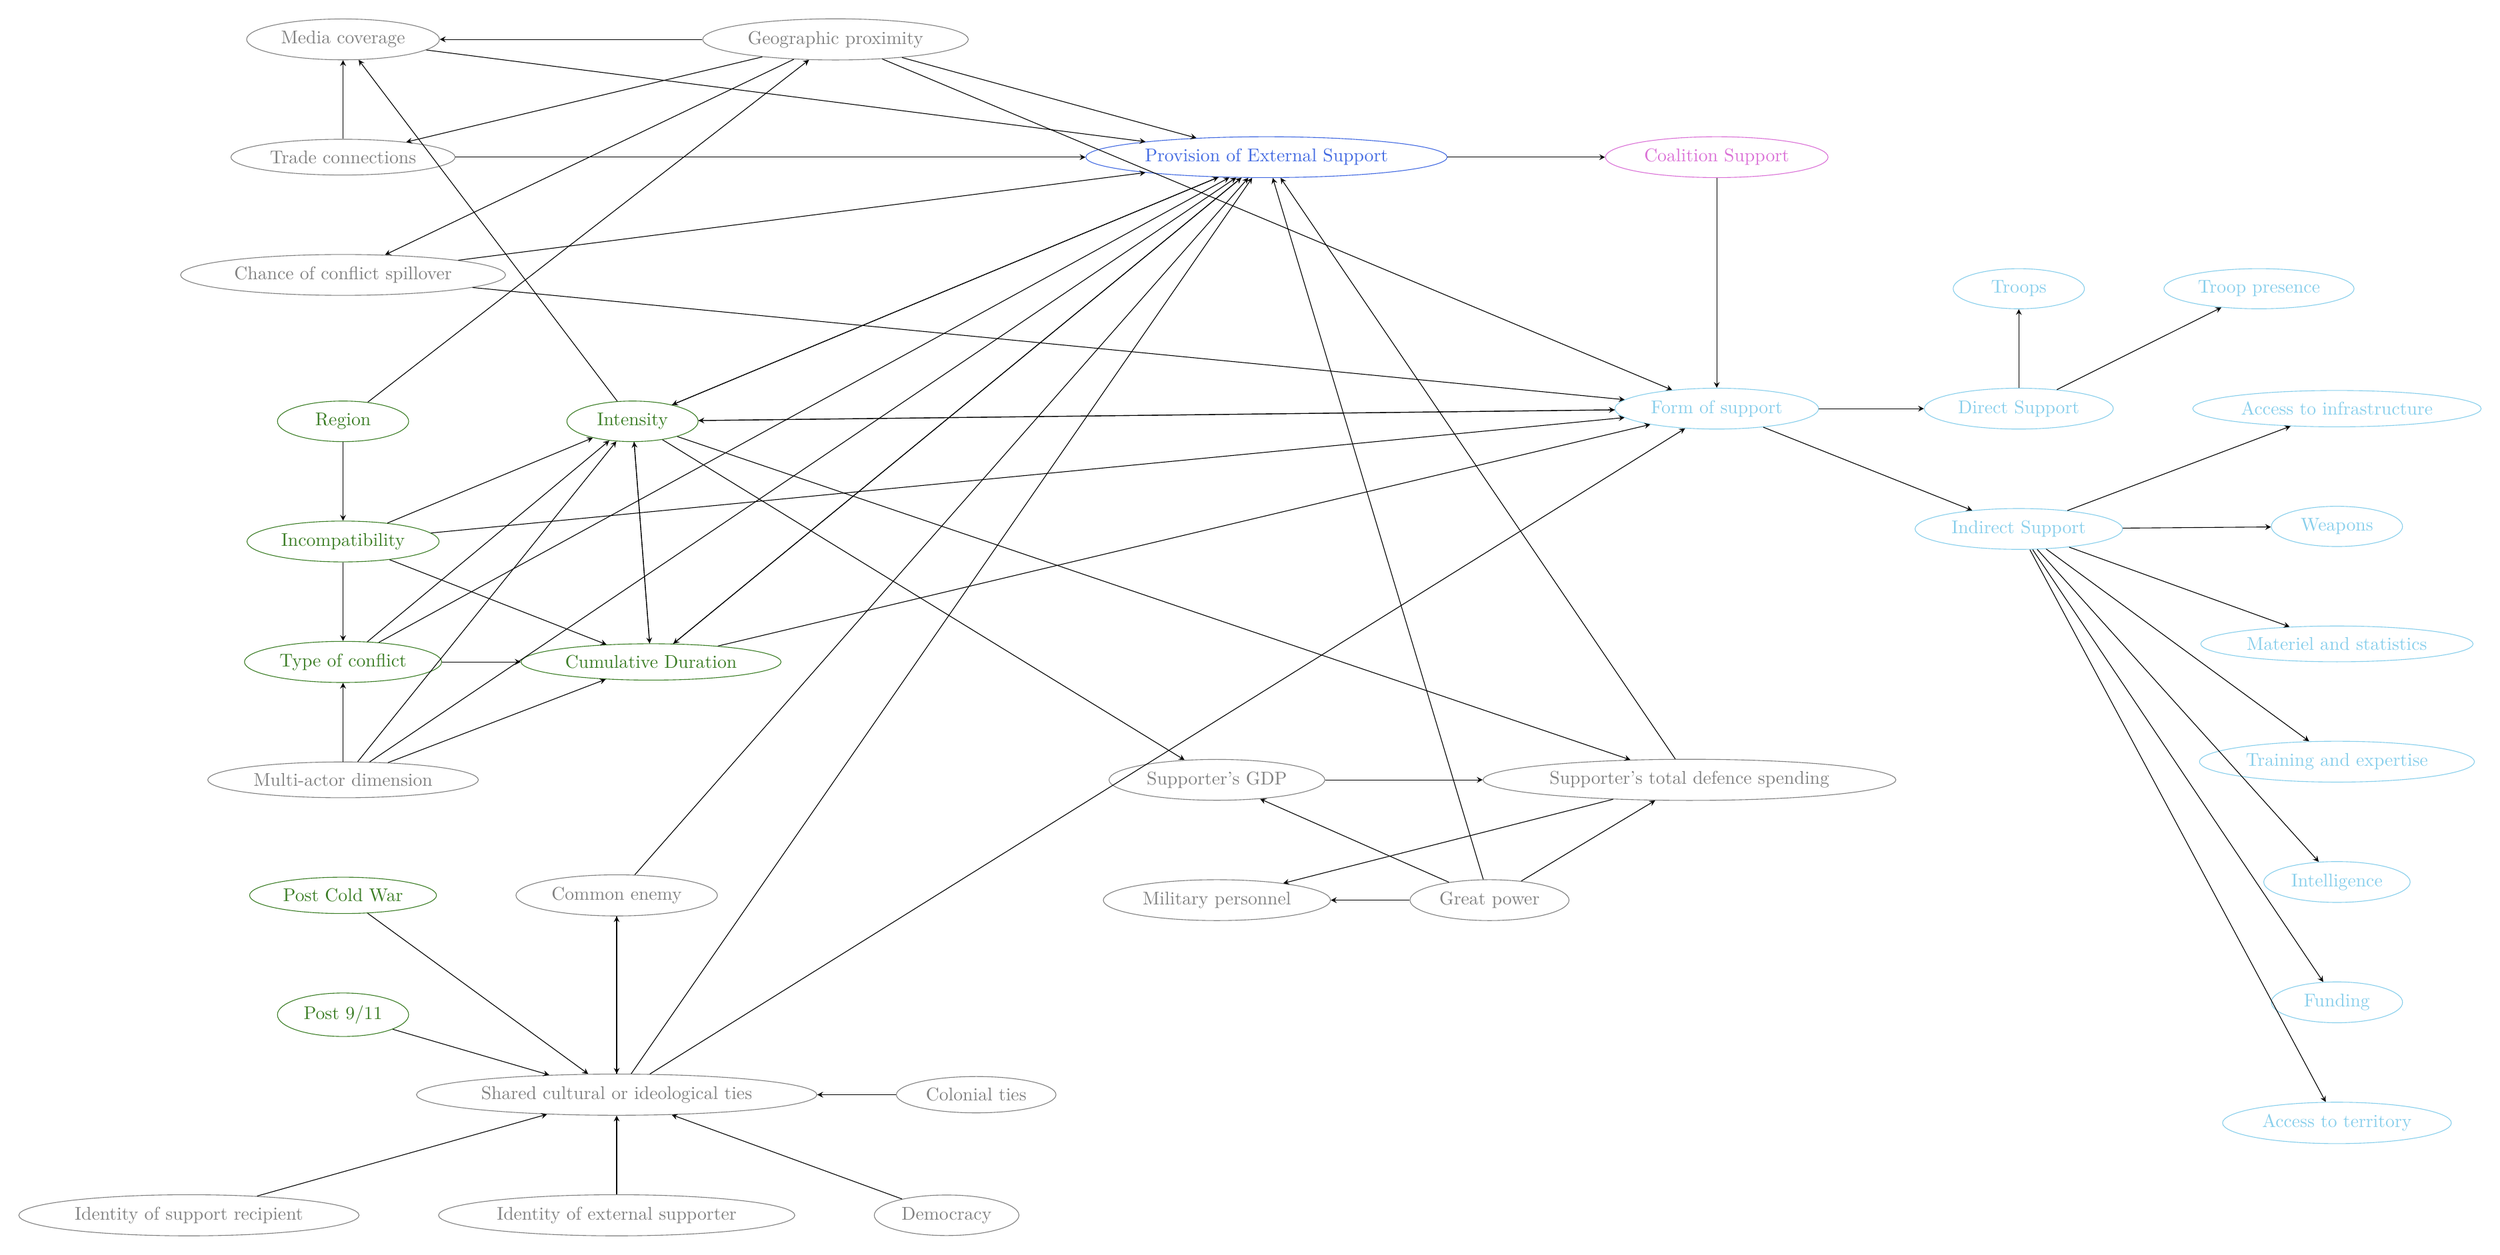
\begin{tikzpicture}[
  scale=1, 
  every node/.style={draw, ellipse, align=center, minimum width=2.5cm}, 
  node distance=1.5cm, 
  ->, >=stealth
]

% Conflict Characteristics and control variables
\node[color = OliveGreen] (incompatibility) {Incompatibility};
\node[below=of incompatibility, color = OliveGreen] (type) {Type of conflict};
\node[above=of incompatibility, color = OliveGreen] (region) {Region};
\node[right=3cm of region, color = OliveGreen] (intensity) {Intensity};
\node[below=of type, color = Gray] (multiactor) {Multi-actor dimension};
\node[right=of type, color = OliveGreen] (duration) {Cumulative Duration};
\node[below=of multiactor, color = OliveGreen] (coldwar) {Post Cold War};
\node[below=of coldwar, color = OliveGreen] (nineeleven) {Post 9/11};
\node[right=of coldwar, color = Gray] (enemy) {Common enemy};
\node[below=3cm of enemy, color = Gray] (culturalties) {Shared cultural or ideological ties};
\node[below=of culturalties, color = Gray] (identityes) {Identity of external supporter};
\node[left=of identityes, color = Gray] (identityrec) {Identity of support recipient};
\node[right=of culturalties, color = Gray] (colonial) {Colonial ties};
\node[right=of identityes, color = Gray] (democracy) {Democracy};

\node[above=2cm of region, color = Gray] (spillover) {Chance of conflict spillover};
\node[above=of spillover, color = Gray] (trade) {Trade connections};
\node[above=of trade, color = Gray] (media) {Media coverage};
\node[right=5cm of media, color = gray] (geography) {Geographic proximity};

\node[right=12cm of multiactor, color = Gray] (GDP) {Supporter's GDP};
    \node[right=3cm of GDP, color = Gray] (defence) {Supporter's total defence spending};
\node[below=of GDP, color = Gray] (military) {Military personnel};
\node[right=of military, color = Gray] (greatpower) {Great power};

% External Support
\node[right=12cm of trade, color = RoyalBlue] (external) {Provision of External Support};
\node[right=3cm of external, color = Orchid] (coalition) {Coalition Support};
\node[below=4cm of coalition, color = SkyBlue] (form) {Form of support};
\node[right=2cm of form, color = SkyBlue] (direct) {Direct Support};
\node[below=of direct, color = SkyBlue] (indirect) {Indirect Support};
\node[above=of direct, color = SkyBlue] (troops) {Troops};
\node[right=of troops, color = SkyBlue] (presence) {Troop presence};
\node[right=of direct, color = SkyBlue] (infrastructure) {Access to infrastructure};
\node[below=of infrastructure, color = SkyBlue] (weapons) {Weapons};
\node[below=of weapons, color = SkyBlue] (logistics) {Materiel and statistics};
\node[below=of logistics, color = SkyBlue] (training) {Training and expertise};
\node[below=of training, color = SkyBlue] (intelligence) {Intelligence};
\node[below=of intelligence, color = SkyBlue] (funding) {Funding};
\node[below=of funding, color = SkyBlue] (territory) {Access to territory};

% Connections
\draw (incompatibility) -- (type);
\draw (incompatibility) -- (intensity);
\draw (incompatibility) -- (duration);
\draw (incompatibility) -- (form);

\draw (type) -- (intensity);
\draw (type) -- (duration);
\draw (type) -- (external);

\draw (intensity) -- (duration);
\draw (duration) -- (intensity);
\draw (intensity) -- (defence);
\draw (intensity) -- (GDP);
\draw (intensity) -- (media);
\draw (intensity) -- (external);
\draw (external) -- (intensity);
\draw (intensity) -- (form);
\draw (form) -- (intensity);

\draw (region) -- (incompatibility);
\draw (region) -- (geography);
\draw (geography) -- (trade);
\draw (geography) -- (media);
\draw (geography) -- (spillover);
\draw (spillover) -- (external);
\draw (spillover) -- (form);
\draw (geography) -- (external);
\draw (geography) -- (form);

\draw (trade) -- (media);
\draw (trade) -- (external);
\draw (greatpower) -- (GDP);
\draw (greatpower) -- (defence);
\draw (greatpower) -- (military);
\draw (greatpower) -- (external);
\draw (defence) -- (military);
\draw (defence) -- (external);
\draw (GDP) -- (defence);

\draw (duration) -- (external);
\draw (external) -- (duration);
\draw (duration) -- (form);

\draw (coldwar) -- (culturalties);
\draw (nineeleven) -- (culturalties);
\draw (identityes) -- (culturalties);
\draw (identityrec) -- (culturalties);
\draw (democracy) -- (culturalties);
\draw (colonial) -- (culturalties);
\draw (culturalties) -- (enemy);
\draw (enemy) -- (culturalties);
\draw (enemy) -- (external);
\draw (culturalties) -- (external);
\draw (culturalties) -- (form);

\draw (multiactor) -- (intensity);
\draw (multiactor) -- (duration);
\draw (multiactor) -- (type);
\draw (multiactor) -- (external);
\draw (media) -- (external);

\draw (external) -- (coalition);
\draw (coalition) -- (form);
\draw (form) -- (direct);
\draw (form) -- (indirect);
\draw (direct) -- (troops);
\draw (direct) -- (presence);
\draw (indirect) -- (infrastructure);
\draw (indirect) -- (weapons);
\draw (indirect) -- (logistics);
\draw (indirect) -- (training);
\draw (indirect) -- (intelligence);
\draw (indirect) -- (funding);
\draw (indirect) -- (territory);

\end{tikzpicture}
}

\captionsetup{justification=raggedright, singlelinecheck=false}
\caption{
\textbf{Figure 1: Directed Acyclic Graph on Conflict Characteristics and External Support.}\\
\textcolor{OliveGreen}{OliveGreen} = Independent variables (H1 and H2); 
\textcolor{Orchid}{Orchid} = Independent variable (H3); 
\textcolor{RoyalBlue}{RoyalBlue} = Dependent variable (H1); 
\textcolor{SkyBlue}{SkyBlue} = Dependent variables (H2 and H3); 
\textcolor{Gray}{Gray} = Not included in the analysis.
}

\end{figure}
\end{landscape}

Based on the outlined Literature, Figure 1 portrays the underlying
assumptions and relationships between conflict characteristics and ES.
Directed Acyclic Graphs visually represent the researcher's theoretical
assumptions about causal mechanisms, sources of bias, and pathways
influencing an outcome, allowing systematic identification of control
variables to estimate causal effects and clarification of relationships
between observed and unobserved variables based on theory and prior
evidence (Fleischer and Diez Roux (2008)). The dependent variable
`provision of ES' is assumed to be both directly and indirectly
influenced by independent conflict characteristics (incompatibility,
type of conflict, intensity, region, cumulative duration, point in time
of the conflict), as well as the identity of the external supporter, the
support recipient and their relationship with one another (i.e.,
colonial ties, shared cultural/ideological ties, a common enemy) and
economic and political factors such as trade connections. These
independent factors are not only assumed to have a direct or indirect
effect on the provision of ES but also on the kind of ES that is
provided to one of the conflict parties. A limitation of this conceptual
model is the absence of temporal dynamics, which could influence the
provision and kind of ES. Despite these limitations, the model provides
a structured framework for testing the hypotheses outlined above.

\section{Methodology}\label{methodology}

\subsection{Data and
operationalisation}\label{data-and-operationalisation}

This study draws on two key datasets from the Uppsala Conflict Data
Program (UCDP): the UCDP Dyadic dataset (Version 18.1) (Harbom et al.
(2008); Pettersson and Eck (2018)) and the UCDP External Support dataset
(ESD) (Version 18.1) (Meier et al. (2023)). The UCDP Dyadic dataset
provides data on ACs, focusing on dyads --- pairs of primary warring
parties --- and spans from 1946 to 2018, with the unit of analysis being
the dyad-year. The dataset includes 2,935 observations across 25
variables, capturing various conflict characteristics such as the type
of conflict, incompatibilities, and combatants. The ESD, covering the
period from 1975 to 2017, focuses specifically on ES provided to
conflict parties, detailing ten types of support such as military
assistance, training, and funding. It offers 2,272 observations of 96
variables, coded from open-source material and subjected to intercoder
reliability checks.

The two datasets were merged using the common identifiers `dyad\_id' and
`year'. Prior to merging, the datasets were checked for uniqueness to
ensure the absence of duplicate rows. The merging process ensured the
removal of duplicates, retaining only the necessary columns for
analysis. The underlying unit of analysis remains the dyad-year. The
final dataset includes 2234 observations of 123 variables on 472 dyads
in 212 conflicts from 1975-2017. The comprehensive information on both
conflict characteristics and characteristics of ES allows the study to
address research questions about the relationship between the two and
the types of support provided by external actors.

Despite their comprehensive nature, these datasets present several
limitations. The availability of data on ES restricts the analysis to
1975--2017, excluding recent geopolitical developments. However, the
period includes major historical phases - such as the Cold War, the
post-Cold War era, and the aftermath of 9/11 - during which ES provision
changed significantly (Testerman (2015); Kalyvas and Balcells (2010) in
Roberts (2019); Meier et al. (2023)). The large sample enables
comparative analysis across time, regions, and conflict types, which
would be difficult to replicate through primary data collection. Still,
UCDP's state-based definition of AC includes only incompatibilities over
government or territory, potentially overlooking underlying causes.
Conflicts with fewer than 25 battle-related deaths per year are
excluded, as are cases with uncertainty around key variables like
incompatibility, actors, or intensity. Geographic precision is also
lacking, as location is defined by the government side in a dyad
(Themnér (2018)) rather than where the conflict occurs. The ESD only
records first-degree supporters - those directly aiding a conflict party
-, while second-degree supporters (e.g., states providing logistical
assistance or funding regional coalitions) are omitted (Meier (2022)).
Although the dataset distinguishes ten types of support, the
categorisation simplifies complex, evolving interactions. Non-state
troop support is consistently coded as zero, and support from
international organisations, diaspora groups, businesses, or religious
institutions is excluded (Meier (2022)). Lastly, the ESD's minimum
threshold for recording assistance may result in underreporting minor
interventions, potentially affecting the accuracy of conclusions about
ES provision.

The study incorporates dependent, independent, and control variables
(Table 1), categorised based on their measurement scales. All nominal
independent variables were factorised to improve analytical clarity.
Conflict characteristics were kept as per their original categorisation,
while cumulative duration was derived using a time-based formula. The
order of conflict type was changed so that `intrastate' instead of
`interstate' would be the reference group to allow for clearer
interpretation in conducted regression analyses. The dependent variables
measuring ES, as defined in the Literature Review (see Meier et al.
(2023); Meier (2022)), were expanded to differentiate between types of
support (ext\_category, ext\_type).

\begin{landscape}
\begingroup\fontsize{7}{9}\selectfont

\begin{longtable}[t]{ll>{\raggedright\arraybackslash}p{6cm}cc}
\caption{\label{tab:Table 1: Variable Table}Table 1: Variables used in the analysis}\\
\toprule
Category & Variable & Description & Measurement Scale & Proportion / Mean\\
\midrule
\endfirsthead
\caption[]{Table 1: Variables used in the analysis \textit{(continued)}}\\
\toprule
Category & Variable & Description & Measurement Scale & Proportion / Mean\\
\midrule
\endhead

\endfoot
\bottomrule
\endlastfoot
Dependent Variables &  &  &  & \\
 & ext\_sup & External support provided (1 = Yes) & Binary & 81.6\\
 & ext\_x & Troop support (1 = Yes) & Binary & 18.93\\
 & ext\_p & Foreign troop presence (1 = Yes) & Binary & 1.97\\
 & ext\_y & Access to infrastructure/joint operations (1 = Yes) & Binary & 22.61\\
\addlinespace
 & ext\_w & Weapons support (1 = Yes) & Binary & 58.59\\
 & ext\_m & Materiel and logistics support (1 = Yes) & Binary & 56.62\\
 & ext\_t & Training and expertise support (1 = Yes) & Binary & 61.59\\
 & ext\_f & Funding support (1 = Yes) & Binary & 46.42\\
 & ext\_i & Intelligence support (1 = Yes) & Binary & 16.43\\
\addlinespace
 & ext\_l & Access to territory (1 = Yes) & Binary & 33.8\\
 & ext\_o & Other support (1 = Yes) & Binary & 7.34\\
 & ext\_u & Unknown support (1 = Yes) & Binary & 4.57\\
 & ext\_category & Categorisation of the form of external support provided (i.e.,  whether no support, one individual form or several forms of support are provided) & Ordinal & 72.65\\
 & ext\_type & Categorisation of external support as direct, indirect, or no support & Nominal & \\
\addlinespace
 &  & Indirect &  & 60.92\\
 &  & Direct &  & 0.98\\
 &  & Direct and indirect &  & 19.07\\
Independent Variables &  &  &  & \\
 & type & Type of conflict (1 = Extrasystemic) & Nominal & \\
\addlinespace
 &  & Intrastate (3) &  & 78.74\\
 &  & Interstate (2) &  & 3.13\\
 &  & Internationalised intrastate (4) &  & 18.13\\
 & intensity & Conflict intensity (1 = Minor conflict, 2 = War) & Binary & 20.1\\
 & incompatibility & Conflict incompatibility & Nominal & \\
\addlinespace
 &  & Territory (1) &  & 45.48\\
 &  & Government (2) &  & 54.03\\
 &  & Territory and government (3) &  & 0.49\\
 & territorial & Conflict incompatibility is about territory (1 = Yes) & Binary & 45.97\\
 & cumulative\_duration & Cumulative years of conflict (Years since first observed conflict year) & Ratio & 7.892\\
\addlinespace
 & region & Region of conflict & Nominal & \\
 &  & Europe (1) &  & 5.33\\
 &  & Middle East (2) &  & 14.28\\
 &  & Asia (3) &  & 37.51\\
 &  & Africa (4) &  & 33.44\\
\addlinespace
 &  & Americas (5) &  & 9.27\\
Control Variables &  &  &  & \\
 & cold\_war & Cold War status (0 = Cold War, 1 = Post-Cold War) & Binary & 58.55\\
 & nine\_eleven & Period relative to 9/11 (0 = Before 9/11, 1 = After 9/11) & Binary & 35\\
 & ext\_coalition & Coalition support (0 = Bilateral support, 1 = Coalition support) & Binary & 6.22\\*
\end{longtable}
\endgroup{}
\end{landscape}

Missing data analysis identified few cases of missing values for the
variables used in the analysis. However, while the underlying data and
computed variables cover most independent factors included in the
theoretical framework outlined above (Figure 1), several important
control variables are missing, as their computation is beyond the scope
of this dissertation. These include geographic proximity, which
influences cross-border spillover effects and logistical feasibility of
support (Federle et al. (2024)), and major power status, as powerful
states are more likely to intervene due to strategic interests (Goldman
and Abulof (2016)). Other omitted factors include military capability
differences, historical adversarial relationships, trade dependencies,
former colonial ties, and the ideological alignment between external
supporters and violent non-governmental organisations (NGOs). The
exclusion of these variables limits the study's ability to fully capture
why certain conflicts receive ES while others do not.

\subsection{Data analysis}\label{data-analysis}

Descriptive statistical methods were employed to summarise and analyse
the data. This included the calculation of total conflict counts per
year, as well as the summarisation of conflict intensity and the mean
and median conflict durations by region. These statistics were
visualised through various graphical methods, providing a clear
depiction of temporal trends in conflict characteristics and support
dynamics.

Regression analysis, utilising random (RE) and fixed effects (FE)
models, was conducted to investigate factors influencing the provision
of various forms of ES in AC. For each form of support, FE and RE
logistic regression models were fitted to test the hypotheses that
conflict characteristics and coalition support influence ES provision.
FE models control for conflict dyad-level heterogeneity by accounting
for within-dyad variation, thus removing time-invariant confounders
specific to each dyad (Huntington-Klein (2023)). In contrast, RE models
assume individual effects are drawn from a random distribution
(typically normal), which allows for estimating both within- and
between-dyad variation, increasing precision and reducing standard
errors (Huntington-Klein (2023)). The decision to include both RE and FE
effects models was driven by the need to account for both within-dyad
and between-dyad variations, as this enables a more comprehensive
assessment of how conflict characteristics influence external support,
addressing both specific within-conflict dynamics and broader patterns
across conflicts. Although hybrid models capturing both dimensions exist
(Fairbrother (2014); Mundlak (1978)), time constraints limited the
analysis to the more conventional FE and RE specifications.

As the dependent variables are binary, binomial logistic regression was
considered the most appropriate approach. However, for robustness, all
support types were initially analysed through four model types: RE
linear, RE logistic, FE linear, and FE logistic. The core independent
variables included incompatibility, conflict type, intensity, cumulative
duration, coalition support, and historical periods such as the
post-Cold War and post-9/11 eras. Region was initially included but
later excluded due to high multicollinearity with conflict type
(Appendix 3), which led to convergence issues in several models.
Preliminary analyses and variable assessment (Table 1) supported the
overall functional validity of the dependent variables. However, the
`incompatibility' variable was recoded to focus on territorial disputes,
avoiding instability caused by low case counts in the combined
`territory and government' category. Following initial estimation,
logistic regression was selected for final interpretation, as it
provided more robust results than linear models across several support
types (Table 3a; Table 3b; Appendix 6). All final models were estimated
based on the corresponding FE or RE logistic regression equations:

FE Logistic Regression: \[
\begin{aligned}
\log \left( \frac{\text{provision of support}}{\text{no provision of support}} \right) =\,
&\alpha + 
\beta_1 \cdot \text{territorial incompatibility} + 
\beta_2 \cdot \text{type} + \\
&\beta_3 \cdot \text{intensity} + 
 \beta_4 \cdot \text{duration} + 
\beta_5 \cdot \text{nine eleven} + \\
&\beta_6 \cdot \text{cold war} + 
\beta_7 \cdot \text{coalition support} + 
\gamma_{\text{dyad\_id}}
\end{aligned}
\]

where
\(\log \left( \frac{\text{provision of support}}{\text{no provision of support}} \right)\)
is the natural logarithm of the odds of the dependent variable
occurring, \(\alpha\) is the intercept, \(\beta\) is the coefficient for
each independent variable, and \(\gamma_{\text{dyad\_id}}\) represents
the fixed effect for each dyad.

RE Logistic Regression: \[
\begin{aligned}
\log \left( \frac{\text{provision of support}}{\text{no provision of support}} \right) =\,
&\alpha_i + 
\beta_1 \cdot \text{territorial incompatibility} + 
\beta_2 \cdot \text{type} + \\
&\beta_3 \cdot \text{intensity} + 
\beta_4 \cdot \text{duration} + 
\beta_5 \cdot \text{nine eleven} + \\
&\beta_6 \cdot \text{cold war} + 
\beta_7 \cdot \text{coalition support}
\end{aligned}
\]

where
\(\log \left( \frac{\text{provision of support}}{\text{no provision of support}} \right)\)
is the natural logarithm of the odds of the dependent variable
occurring, \(\alpha_i\) is the intercept varying between dyads (i), and
\(\beta\) is the coefficient for each independent variable.

Both RE and FE models for the overall provision of support, troop
support, and foreign troop presence failed to converge and were
consequently re-estimated using Poisson Pseudo Maximum Likelihood (PPML)
models.\footnote{PPML is widely endorsed in the methodological
  literature for producing consistent estimates under conditions where
  logistic models with FE often encounter separation or quasi-complete
  separation issues (Silva and Tenreyro (2006)). It is also robust to
  heteroscedasticity and handles high-dimensional FE efficiently - an
  important feature for longitudinal dyadic conflict data (Correia et
  al. (2020)). Given these advantages, PPML offers a methodologically
  sound alternative to logistic regression in contexts prone to
  convergence problems.} The refitted PPML models used the same set of
independent variables as the logistic regressions, with the dependent
variable defined as the provision of each respective form of external
support and were estimated using the following equations:

FE PPML Regression: \[
\begin{aligned}
\mathbb{E}(Y_{i} \mid X_{i}, \gamma_i) = \exp\bigg(&
\gamma_i + 
\beta_1 \cdot \text{Territorial Incompatibility}_{i} + 
\beta_2 \cdot \text{Type}_{i} + \\
&\beta_3 \cdot \text{Intensity}_{i} + 
\beta_4 \cdot \text{Duration}_{i} + 
\beta_5 \cdot \text{Post 9/11}_{i} + \\
&\beta_6 \cdot \text{Cold War}_{i} + 
\beta_7 \cdot \text{Coalition Support}_{i}
\bigg)
\end{aligned}
\]

\(\mathbb{E}(Y_{it} \mid X_{it}, \gamma_i)\) is the expected count
outcome (e.g.~probability of receiving support) for unit i and
\(\gamma_i\) represents the dyad-specific fixed effects. The
exponentiation is key to PPML, as the model estimates log-linear
coefficients using a Poisson-based pseudo-likelihood, even when the
dependent variable is not truly count data. Different to the RE model,
\(\gamma_i\) is treated as a parameter to be estimated, rather than a
random draw from a distribution.

RE PPML Regression: \[
\begin{aligned}
\mathbb{E}(Y_{i} \mid X_{i}, \alpha_i) = \exp\bigg(&
\alpha_i + 
\beta_1 \cdot \text{Territorial Incompatibility}_{i} + 
\beta_2 \cdot \text{Type}_{i} + \\
&\beta_3 \cdot \text{Intensity}_{i} + 
\beta_4 \cdot \text{Duration}_{i} + 
\beta_5 \cdot \text{Post 9/11}_{i} + \\
&\beta_6 \cdot \text{Cold War}_{i} + 
\beta_7 \cdot \text{Coalition Support}_{i}
\bigg)
\end{aligned}
\]

where \(\mathbb{E}(Y_{it} \mid X_{it}, \alpha_i)\) is the expected count
outcome (e.g.~probability of receiving support) for unit i, conditional
on covariates and random effect, and \(\alpha_i\) is the dyad-specific
random effect. These analyses provide an overview of trends in the
provision of ES without making inferential claims about causal
relationships.

Due to persistent non-convergence in the FE model for troop presence,
particularly with the 9/11 variable, this variable was removed to ensure
model convergence. While ensuring a working model, it prevents analysis
of 9/11's effect on troop presence and comparison with other models.
Model fit was assessed throughout using the Bayesian Information
Criterion (BIC), Akaike Information Criterion (AIC) for RE models, and
Adjusted Pseudo R-Squared for FE models, with lower values indicating
better fit (Gelman and Hill (2006)). Recoding the incompatibility
variable to focus on territorial disputes and removing the region
variable had no effect on FE BIC values but slightly increased AIC and
BIC in RE models. Despite the marginal decline in model fit, these
adjustments were necessary for convergence. Similarly, refitting models
for troop support and foreign troop presence as PPML led to higher BIC
values, but the approach was retained as it enabled model estimation.

An overall comparison of conflict characteristics' effects on ES was
conducted between and within conflicts, with troop support and
intelligence models selected for detailed analysis. These were chosen
due to the strength of their associations with conflict characteristics
in either the RE or FE models. They also enabled exploration of how
different conflict characteristics correlate with the provision of
direct versus indirect support. However, the use of distinct model types
across support forms (due to convergence issues) limits the direct
comparability between direct and indirect support provisions.

Logistic regression results were interpreted using odds ratios,
reflecting the change in odds of receiving support for a one-unit
increase in the predictor. PPML results were interpreted through
incidence rate ratios (IRR), indicating the change in expected count of
ES provision for a one-unit increase in the independent variable. While
the dependent variables are binary, PPML models treat them as count
variables---an accepted compromise to allow valid estimation. To enhance
interpretability, logistic regression coefficients were exponentiated.
Despite discussions on redefining statistical significance (Benjamin et
al. (2018)), this report rejects the null hypothesis that the
population's estimated coefficient is zero when p \textless.05.
Multicollinearity was not expected due to the distinct nature of the
conflict characteristics. Nevertheless, variance inflation factors
(VIFs) were calculated for RE models where applicable. Standard
regression assumptions were tested across models to ensure validity and
reliability. However, as most predictors were categorical, the linearity
assumption did not apply to them, and due to the logistic nature of the
models, homoscedasticity and residual normality were not relevant.

\section{Findings}\label{findings}

\subsection{Overall trends in conflict
characteristics}\label{overall-trends-in-conflict-characteristics}

Although the total number of conflicts has decreased and minor ACs make
up the majority of ACs, recent years have seen a rise in wars (Figure
2).

\includegraphics{Dissertation_writeup_files/figure-latex/Figure 2: Intensity-1.pdf}

While most conflicts are fought in Asia and Africa, the number of
conflicts fought in the Middle East is growing (Appendix 1), with
conflicts in Asia and the Americas portraying longer duration (Figure
3).

\includegraphics{Dissertation_writeup_files/figure-latex/Figure 3: Duration-1.pdf}

Intrastate conflicts are the most common type of conflict, followed by
internationalised intrastate conflicts, whose number has been growing
since the early 2000s (Appendix 2). While there is fluctuation between
the incompatibility types `territory' and `government', most conflicts
in 2017 were about territory and hardly any about territory and
government (Appendix 4).

\subsection{The provision of external
support}\label{the-provision-of-external-support}

The provision of ES has risen, with indirect support being the most
common (Figure 4) and supporters providing three forms of support on
average (Median: 4). The provision of support in a coalition has
increased over time (Appendix 5).

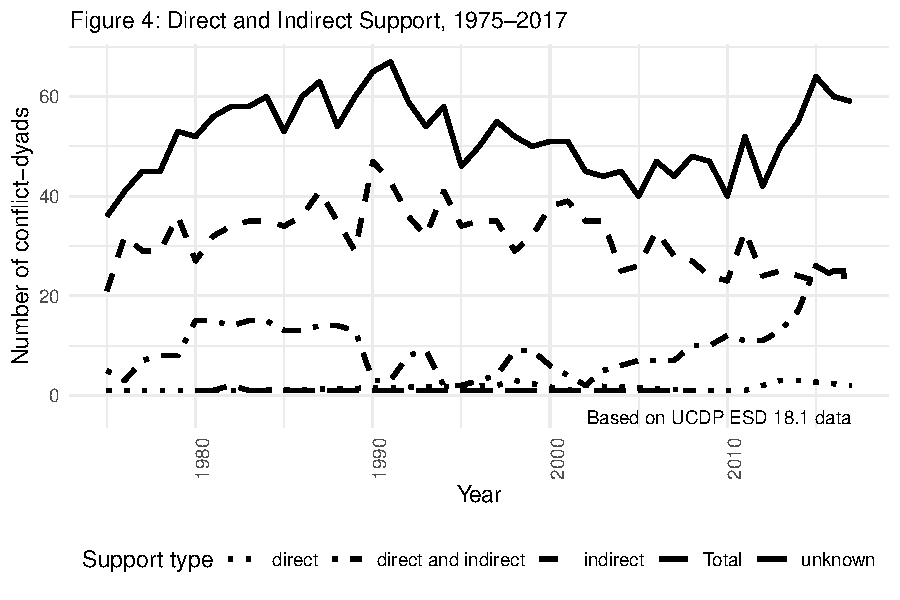
\includegraphics{Dissertation_writeup_files/figure-latex/Figure 4 (In-)direct support-1.pdf}

The models for the provision of ES (Table 2) show no statistically
significant results. However, the results of the regression analyses for
individual forms of support reveal distinct patterns in the relationship
between conflict characteristics and the provision of ES, with notable
differences between RE and FE models.

\newpage

\noindent\textbf{Table 2: Regression Results – External Support Determinants}

\begin{tabular}{lll}
\hline
& Random Effects (PPML) & Fixed Effects (PPML) \\ \hline
(Intercept) & \num{1.000} &  \\
& [\num{0.890}, \num{1.124}] &  \\
Type (interstate) & \num{1.003} &  \\
& [\num{0.657}, \num{1.531}] &  \\
Type (internationalised intrastate) & \num{1.005} & \num{1.005} \\
& [\num{0.873}, \num{1.157}] & [\num{0.996}, \num{1.015}] \\
Num.Obs. & \num{1451} & \num{1449} \\
R2 &  & \num{0.002} \\
R2 Adj. &  & \num{-0.220} \\
R2 Within &  & \num{0.000} \\
R2 Within Adj. &  & \num{-0.004} \\
AIC & \num{2921.6} & \num{3538.7} \\
BIC & \num{2974.4} & \num{5248.9} \\
RMSE & \num{0.10} & \num{0.07} \\
Std.Errors &  & by: dyad\_id \\
FE: dyad\_id &  & X \\
\hline
\end{tabular}

In the RE logistic regression (Table 3a), the type of conflict ---
particularly internationalised intrastate conflicts --- emerges as
strongly correlated to the provision of ES, showing significance in
seven of the nine models. Other influential factors include conflict
intensity and the post-Cold War period, which are strongly correlated
with multiple forms of support. Intelligence provision appears to be the
most sensitive to conflict characteristics, with six out of seven
independent variables reaching statistical significance. Medium-level
correlations are observed for access to infrastructure, weapons,
materiel and logistics, training and expertise, and funding, while troop
support and troop presence exhibit the weakest correlations. While troop
support was correlated to the type of conflict, troop presence was
correlated to the post-Cold War and post-9/11 eras.

\begin{landscape}
\begin{table}[!h]
\centering
\caption{\label{tab:Tables 3: RE and FE logistic regression - statistical significance}Table 3a: Statistical Significance in the RE Logistic Regression Models}
\centering
\resizebox{\ifdim\width>\linewidth\linewidth\else\width\fi}{!}{
\fontsize{8}{10}\selectfont
\begin{tabular}[t]{lccccccccc}
\toprule
Independent Variable & Troop Support & Troop Presence & Access to Infrastructure & Weapons & Materiel and Statistics & Training and Expertise & Funding & Intelligence & Access to Territory\\
\midrule
Intercept & *** & *** & *** & *** & *** & *** &  & *** & **\\
Territorial dispute &  &  &  &  & . &  &  & . & \\
Type of conflict & *** (Interstate); *** (Internationalised intrastate) &  & ** (Internationalised intrastate) & * (Internationalised intrastate) & ** (Internationalised intrastate) & * (Interstate); * (Internationalised intrastate) & * (Interstate); * (Internationalised intrastate) &  & . (Interstate)\\
Intensity &  & . (War) &  & *** (War) & *** (War) &  & *** (War) & * (War) & \\
Duration &  &  & * &  &  & . & . & * & \\
\addlinespace
9/11 &  & * (After) &  & * (After) &  & * (After) &  & *** (After) & \\
Cold War &  &  & *** (After) & *** (After) & * (After) & ** (After) & ** (After) & ** (After) & . (After)\\
Coalition Support &  &  & *** (Coalition) &  &  &  & . (Coalition) & * (Coalition) & ** (Coalition)\\
N & 1451 & 1451 & 1451 & 1451 & 1451 & 1451 & 1451 & 1451 & 1451\\
AIC & 949.6 & 326.5 & 1250.3 & 1094.5 & 1210.8 & 1066.9 & 1317.5 & 922.5 & 1294.9\\
\addlinespace
BIC & 1002.4 & 379.3 & 1303.1 & 1147.3 & 1263.6 & 1119.7 & 1370.3 & 975.3 & 1347.7\\
\bottomrule
\end{tabular}}
\end{table}
\vspace{1cm}
\begin{table}[!h]
\centering
\caption{\label{tab:Tables 3: RE and FE logistic regression - statistical significance}Table 3b: Statistical Significance in the FE Logistic Regression Models}
\centering
\resizebox{\ifdim\width>\linewidth\linewidth\else\width\fi}{!}{
\fontsize{8}{10}\selectfont
\begin{tabular}[t]{lccccccccc}
\toprule
Independent Variable & Troop Support & Troop Presence & Access to Infrastructure & Weapons & Materiel and Statistics & Training and Expertise & Funding & Intelligence & Access to Territory\\
\midrule
Type of conflict & *** (Internationalised intrastate) &  &  &  &  & . (Internationalised intrastate) &  &  & \\
Intensity &  &  &  & * (War) & . (War) &  & * (War) & . (War) & \\
Duration &  &  &  & * &  &  & * & . & \\
9/11 &  & *** (After) &  & * (After) &  &  &  &  & . (After)\\
Cold War &  & *** (After) &  & . (After) &  & . (After) &  & * (After) & \\
\addlinespace
Coalition Support &  &  &  &  &  &  &  &  & \\
N & 646 & 181 & 612 & 557 & 603 & 515 & 683 & 513 & 681\\
BIC & 1625.5 & 328.1 & 1074.7 & 949.6 & 1051.2 & 885.2 & 1128.9 & 795.6 & 1113.8\\
Adjusted Pseudo R-squared & 0.09521 & -0.021449 & 0.04485 & 0.157779 & 0.071311 & 0.030282 & 0.179317 & 0.208345 & 0.169719\\
\bottomrule
\end{tabular}}
\end{table}
\end{landscape}

Within conflicts, as captured by the FE models (Table 3b), the provision
of ES is overall less correlated to conflict characteristics than in the
comparison between conflicts (RE). The era post-Cold War, as well as
conflict intensity, show the most significance across FE models.
However, conflict intensity is correlated with the provision of indirect
ES but not with the provision of direct support. The provision of
weapons and intelligence are correlated with most conflict
characteristics, with conflict intensity, duration, and the post-Cold
War era being significant in both. The provision of troop support is
only correlated to the type of conflict, while troop presence is
correlated to conflict duration. Access to infrastructure is not
correlated to any conflict characteristics and the provision of materiel
and statistics, training and expertise, funding, and access to territory
are only correlated to one or two conflict characteristics.

All models were tested against standard regression assumptions to ensure
validity and reliability. UCDP data was deemed appropriate for
addressing the research questions, as it comprehensively captures AC and
ES characteristics, although empirical datasets rarely meet all
theoretical criteria perfectly (Gelman and Hill (2006)). Table 1
confirmed the functionality of the dependent variables.
Multicollinearity was assessed in RE models using VIFs, with all values
below 5, indicating no significant collinearity issues (O'Brien (2007)).
As most predictors were categorical, the linearity assumption did not
apply. For the sole continuous variable, cumulative duration, linearity
was assessed where possible (RE models). The assumption of independent
errors was violated due to repeated observations per conflict and dyad.
Homoscedasticity and residual normality were not applicable to logistic
models. The binary nature of the dependent variable confirmed the
appropriateness of logistic regression for the analysis.

\section{Discussion}\label{discussion}

The findings of this study align with existing literature on conflict
dynamics and external interventions. Over time, the number of wars has
slightly increased, indicating a shift towards more intense conflicts,
while conflict duration has increased, suggesting that many conflicts
persist rather than being resolved. These trends are consistent with
research highlighting the protracted nature of modern ACs (Quinn et al.
(2007)). The nature of ES has also evolved. While troop support has
declined, the total number of external interventions continues to rise
(Figure 4), demonstrating a persistent strategic interest in shaping
conflict trajectories through both direct and indirect means (Davies et
al. (2024); Chang and Sellak (2022)). Recent years have seen a shift
toward multilateral coalitions and collaborative interventions (Appendix
5), with nearly one-third of all support instances involving such
coalitions, reflecting a greater emphasis on burden-sharing and
legitimacy (Meier et al. (2023)).

The findings from the regression analysis suggest that while structural
conflict factors are correlated to the provision of ES, temporal and
contextual elements play a decisive role within individual conflicts.
This aligns with existing literature on the provision of ES, which
emphasises the importance of conflict characteristics in shaping
external intervention strategies (Berlin and Malone (2023); Davies et
al. (2024)). While the models examining HG1 show no statistically
significant results, regression analyses for individual forms of support
reveal distinct patterns in the relationship between conflict
characteristics and the provision of ES, with notable differences
between the RE and FE models.

RE models show that the provision of indirect support is more correlated
to conflict characteristics than direct support, with intelligence
provision being the most sensitive to these factors. This finding aligns
with existing literature suggesting that indirect forms of support are
often more prevalent in contemporary conflicts (Meier et al. (2023);
Berlin and Malone (2023)). Especially the provision of intelligence is
strongly correlated with conflict characteristics, suggesting that
external actors tailor intelligence support to specific conflict
dynamics rather than adopting a one-size-fits-all approach. While no
trends could be discovered in the provision of direct forms of support
and the correlation to different conflict characteristics of troop
presence and troop support might seem counter intuitive at first, it
could indicate an escalation in the provision of ES with the former
being a precondition for the latter. Conflict intensity (RE), and the
post-Cold war era, as well as conflict duration (FE) might be first
incentives for external supporters to provide more direct support but
once troops are already present, the type of conflict might then become
a more important factor in the decision to provide troop support.
Therefore, HG1 cannot be completely rejected but the results rather
indicate that the provision of ES is not only correlated to conflict
characteristics but that it may further be dependent on the form of
support provided.

For HG2, which explores whether conflict characteristics influence the
type of ES provided, results reveal that conflict intensity (H2a) is
significantly correlated to the provision of weapons, materiel and
statistics, funding, and intelligence in both FE and RE models. This
aligns with the argument that higher-intensity conflicts are more likely
to receive ES due to concerns about spillover effects and escalation
(Cunningham (2010); Gregory (2000)). However, intensity does not appear
to significantly impact the provision of troop support, suggesting that
external actors may not relate the intensity of a conflict to increased
levels of direct support.

Besides intensity, the provision of access to infrastructure, weapons,
materiel and statistics, training and expertise, funding, and access to
territory show consistent correlations with conflict duration (H2c), the
type of conflict (H2d), and whether a conflict is taking place after
9/11 (H2e) or after the Cold War (H2f) in the RE models. Particularly
internationalised intrastate conflicts are strongly correlated with the
provision of ES. Within a conflict, conflict intensity, duration, and
the post-Cold War era seem to be more correlated with the provision of
indirect ES. These findings are consistent with prior research
suggesting that the Cold War significantly shaped patterns of external
intervention. During this period, superpowers engaged in proxy
conflicts, fueling insurgencies and prolonging wars, whereas the
post-Cold War era saw a shift towards more selective and strategic forms
of ES (Testerman (2015); Kalyvas and Balcells (2010) in Roberts (2019)).
The significance of the periods after the Cold War and 9/11, and
conflict intensity in both FE and RE models, suggests that broader
geopolitical shifts and conflict dynamics may play a crucial role in
shaping ES provision, whether within one ongoing or between different
conflicts. This divergence highlights the complexity of ES dynamics and
suggests that different forms of support may be influenced by different
factors.

On the other hand, territorial incompatibility (H2b) is not
significantly correlated with the provision of most ES, suggesting that
this factor plays a less prominent role in shaping external intervention
strategies. The lack of significant correlations between territorial
incompatibility with ES provision is surprising, as previous research
has highlighted the importance of this factor in shaping conflict
dynamics and external interventions (Cunningham (2010); Gregory (2000)).
The absence of a significant relationship between cumulative conflict
duration and the provision of support further challenges assumptions
that protracted conflicts necessarily attract sustained external
intervention.

Findings suggest that coalition support (H3) is significantly associated
with access to infrastructure, funding, intelligence, and access to
territory in the RE model. However, in the FE model, it shows no
statistical significance at all. This suggests that coalition dynamics
play a more prominent role in shaping the types of ES provided across
different conflicts than within individual conflicts.

Model-specific results further illustrate these patterns: troop support
is most strongly correlated to the type of conflict, whereas
intelligence provision shows broader but less consistent correlations
with conflict characteristics. Already presented in Table 3, these
models were selected for detailed analysis to explore how different
conflict characteristics correlate with the provision of direct versus
indirect support. In the RE model (Table 4a), the IRR of foreign troop
support is 13.79 units higher for interstate conflicts, and 72.77 units
higher for internationalised intrastate conflicts compared to intrastate
conflicts, holding all other conflict characteristics constant. Due to
issues with collinearity, the category of interstate conflicts was
excluded from the FE model (Table 4b), making a comparison impossible.
The average IRR of troop support for internationalised intrastate
conflicts is 70.27 units higher than for intrastate conflicts, holding
all other factors constant. The closeness of coefficients between the RE
and FE models suggests that conflict type has roughly the same effect on
the provision of troop support, both between and within conflicts. This
suggests that the type of conflict could be a significant factor in
determining the provision of troop support, with interstate and
internationalised intrastate conflicts being more likely to receive this
form of support than intrastate conflicts. The significance of
especially internationalised intrastate conflicts might be explained by
the fact that they are often more complex and involve multiple actors,
which creates opportunities for external actors to provide support to
one side or another, depending on their interests and objectives.

\newpage

\noindent\textbf{Table 4a: RE Logistic and PPML Regression Results}

\begin{tabular}{lll}
\hline
& Troop Support (RE PPML) & Intelligence (RE Logit) \\ \hline
(Intercept) & \num{0.014}*** & \num{0.000}*** \\
& [\num{0.008}, \num{0.026}] & [\num{0.000}, \num{0.002}] \\
Type (interstate) & \num{13.792}*** & \num{2.740} \\
& [\num{4.431}, \num{42.930}] & [\num{0.077}, \num{97.090}] \\
Type (internationalised intrastate) & \num{72.768}*** & \num{2.172} \\
& [\num{41.080}, \num{128.897}] & [\num{0.835}, \num{5.646}] \\
Num.Obs. & \num{1451} & \num{1451} \\
R2 Marg. &  & \num{0.140} \\
R2 Cond. &  & \num{0.922} \\
AIC & \num{949.6} & \num{922.5} \\
BIC & \num{1002.4} & \num{975.3} \\
ICC &  & \num{0.9} \\
RMSE & \num{0.11} & \num{0.23} \\
\hline
\end{tabular}

\noindent\textbf{Table 4b: FE Logistic and PPML Regression Results}

\begin{tabular}{lll}
\hline
& Troop Support (FE PPML) & Intelligence (FE Logit) \\ \hline
Type (internationalised intrastate) & \num{70.265}*** & \num{1.686} \\
& [\num{19.269}, \num{256.225}] & [\num{0.287}, \num{9.925}] \\
Num.Obs. & \num{646} & \num{513} \\
R2 & \num{0.295} & \num{0.361} \\
R2 Adj. & \num{0.091} & \num{0.208} \\
R2 Within & \num{0.174} & \num{0.190} \\
R2 Within Adj. & \num{0.162} & \num{0.168} \\
AIC & \num{1080.1} & \num{562.4} \\
BIC & \num{1625.5} & \num{795.6} \\
RMSE & \num{0.10} & \num{0.38} \\
Std.Errors & by: dyad\_id & by: dyad\_id \\
FE: dyad\_id & X & X \\
\hline
\end{tabular}

For intelligence support, both models find that the odds for wars are
lower than that for minor ACs to receive this form of aid (odds = 0.44
in RE; 0.33 in FE), holding all other factors constant. Both models
further indicate that conflicts occurring after the Cold War are
correlated with the provision of intelligence, although the effect is
stronger in the FE model (odds = 8.41) than in the RE model (odds =
6.4). The odds of receiving intelligence support increase with each year
in conflict duration (by 1.06 in RE and 1.12 in FE models). While the RE
model suggests that intelligence provision is correlated to the time
period after 9/11 (odds = 8.27) and coalition support (odds = 4.49),
holding all other variables constant, these effects do not emerge as
statistically significant in the FE model. These results could suggest
that external actors tailor intelligence support to specific conflict
dynamics and supporting the notion that intelligence-sharing plays a
crucial role in modern conflict interventions, allowing external
supporters to shape conflict outcomes strategically (Schultz (2010);
Bapat (2012); Sawyer et al. (2015)). The findings highlight key
theoretical implications for Criminology and conflict studies. The weak
correlation between direct support and conflict characteristics suggests
that direct military interventions may be driven by factors beyond
conflict characteristics alone, such as diplomatic or geopolitical
considerations.

The inability to control for regional variation or geographic proximity
limits the generalisability of the findings, as well as their
interpretation from a criminological perspective. Tobler (1970) law,
`everything is related to everything else, but near things are more
related than distant things' suggests that geographic proximity may play
a significant role in shaping the dynamics of ES. Not controlling for
geographic proximity might thereby ignore important contextual factors
that influence the provision of ES. Despite this, the results confirm
existing theories that ES provision is influenced by conflict
characteristics---particularly intensity and duration---yet also
underscore that different forms of support respond to these
characteristics in distinct ways. This supports a `cold logic'
interpretation, in which state actors rationally assess the strategic
value of conflict before engaging, rather than reacting emotionally.
This aligns with prior research suggesting intervention decisions are
based on a rational assessment of costs, benefits, and political
alignment (Schultz (2010); Bapat (2012); Sawyer et al. (2015)). However,
the absence of data on shared cultural ties or geographic proximity
prevents assessment of whether certain interventions also follow a `hot'
logic, where emotional or identity-driven factors---such as shared
ethnicity or history---play a role. This opens an important avenue for
future research that more explicitly incorporates emotional, symbolic,
and identity-based motivations.

Further limitations arise from the dataset's focus on state-based
conflicts, which omits the growing influence of non-state actors and
transnational networks in modern conflict. Additionally, provider and
recipient characteristics---key to understanding the criminological
dynamics of power, ideology, and legitimacy---could not be tested due to
data constraints. Reverse causality also poses a risk: rather than
resolving conflict, ES may prolong it by altering the incentives for
continued violence (Fearon (2004) in Testerman (2015); Lacina (2006)).
While model refitting and variable exclusion (i.e., 9/11 in the FE model
for foreign troop presence) were necessary to achieve convergence, these
changes limit comparability across models. The exclusive use of
quantitative methods further restricts insight into the lived
experiences and micro-level effects of ES. Future research should
therefore enhance this study by incorporating qualitative data and case
studies to provide a more comprehensive understanding of the
relationship between ES and conflict dynamics.

\section{Conclusion}\label{conclusion}

This study set out to examine how characteristics of AC shape the
provision of ES, offering new insights into the strategic logic
underlying state interventions. Contemporary examples such as Russia's
invasion of Ukraine, evidence the limitations of pacifist responses. But
while military interventions can at times stabilise volatile regions,
they often risk escalating violence or prolonging conflict (Fearon
(2004) in Testerman (2015); Lacina (2006); Olson Lounsbery (2016)). The
findings show that ES---particularly indirect forms---is significantly
influenced by conflict characteristics, suggesting a calculated, `cold'
approach to intervention. Rather than being random or purely
humanitarian, ES appears to reflect strategic assessments of conflict
dynamics, reinforcing existing literature on the instrumental use of
support in warfare (Schultz (2010); Bapat (2012); Sawyer et al. (2015)).
Crucially, the type of support provided varies with conflict
characteristics, indicating that ES is not a one-size-fits-all strategy.
These results have important implications for criminology. If states
make informed, strategic decisions to intervene in armed conflicts, they
may bear greater responsibility for the violence and crimes that unfold
in these contexts. Yet, this dimension of liability and complicity
remains underexplored in criminological research. This study offers a
starting point for engaging with ES as a site of criminological concern,
where questions of accountability, harm, and power intersect. By
broadening its focus to include the indirect consequences of state
interventions, criminology can contribute to more effective policy
responses and a deeper understanding of the global production and
regulation of violence.

\section{Appendices}\label{appendices}

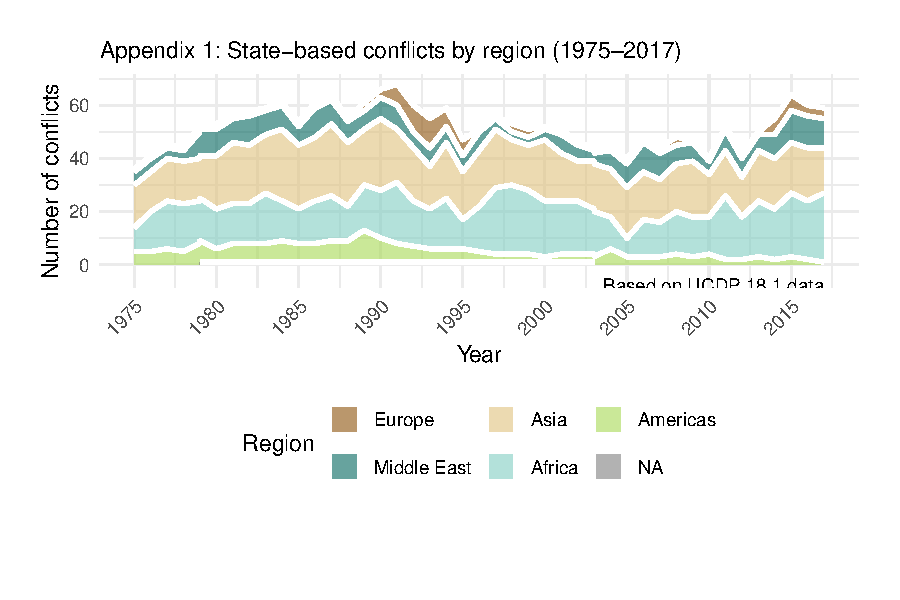
\includegraphics{Dissertation_writeup_files/figure-latex/Region (Appendix 1)-1.pdf}

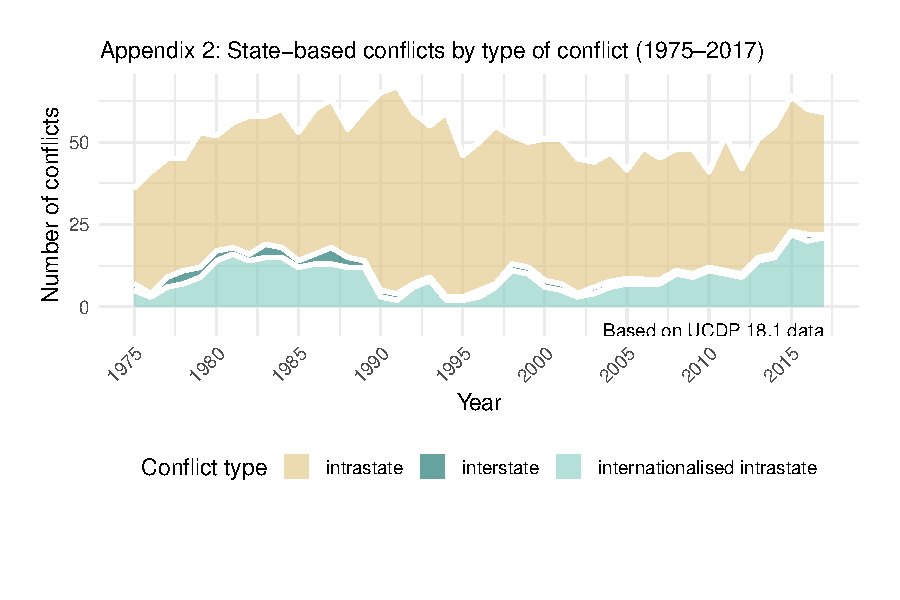
\includegraphics{Dissertation_writeup_files/figure-latex/Conflict type (Appendix 2)-1.pdf}

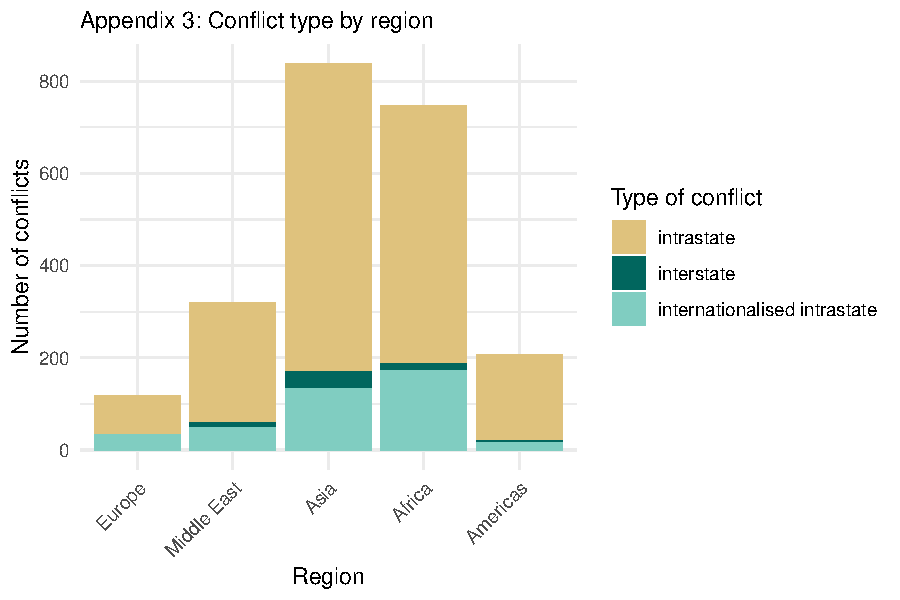
\includegraphics{Dissertation_writeup_files/figure-latex/Bivariate analysis between conflict type and region (Appendix 3)-1.pdf}

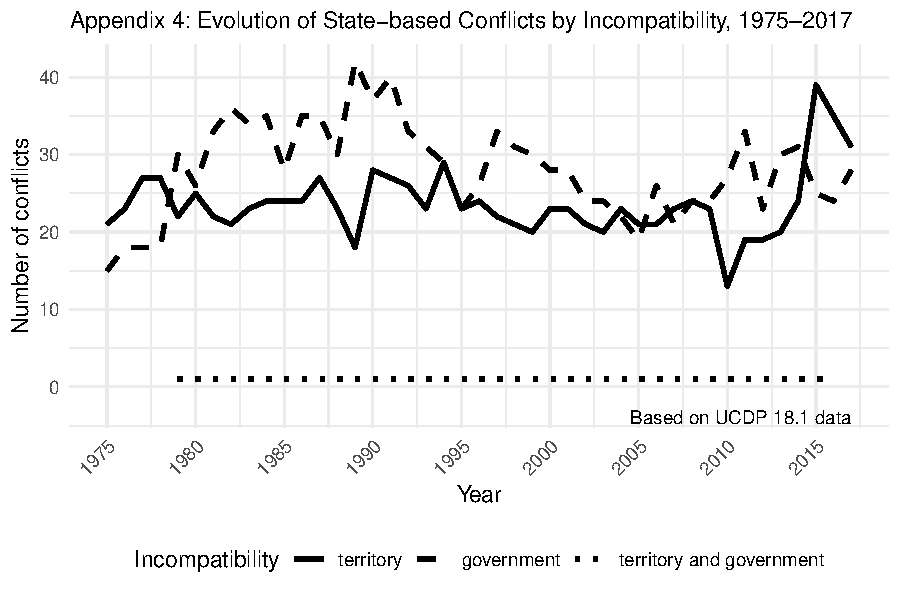
\includegraphics{Dissertation_writeup_files/figure-latex/Incompatibility (Appendix 4)-1.pdf}

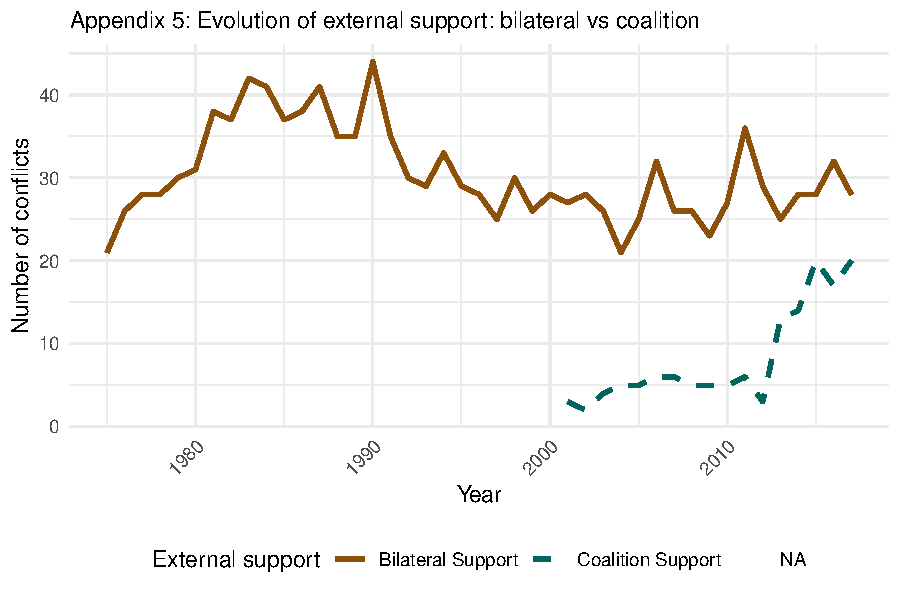
\includegraphics{Dissertation_writeup_files/figure-latex/Coalition Support (Appendix 5)-1.pdf}

\begin{landscape}\begin{table}[!h]
\centering
\caption{\label{tab:Table Random effects linear regression - statistical significance (Appendix 6)}Appendix 6: Statistical Significance in the RE Linear Regression models}
\centering
\resizebox{\ifdim\width>\linewidth\linewidth\else\width\fi}{!}{
\fontsize{7}{9}\selectfont
\begin{tabular}[t]{lccccccccc}
\toprule
Independent Variable & Troop Support & Troop Presence & Access to Infrastructure & Weapons & Materiel and Statistics & Training and Expertise & Funding & Intelligence & Access to Territory\\
\midrule
Intercept & *** & *** & *** & *** & *** & *** &  & *** & **\\
Territorial dispute &  &  &  &  & . &  &  & . & \\
Type of conflict & *** (Interstate); *** (Internationalised intrastate) &  & ** (Internationalised intrastate) & * (Internationalised intrastate) & ** (Internationalised intrastate) & * (Interstate); * (Internationalised intrastate) & * (Interstate); * (Internationalised intrastate) &  & . (Interstate)\\
Intensity &  & . (War) &  & *** (War) & *** (War) &  & *** (War) & * (War) & \\
Duration &  &  & * &  &  & . & . & * & \\
\addlinespace
9/11 &  & * (After) &  & * (After) &  & * (After) &  & *** (After) & \\
Cold War &  &  & *** (After) & *** (After) & * (After) & ** (After) & ** (After) & ** (After) & . (After)\\
Coalition Support &  &  & *** (Coalition) &  &  &  & . (Coalition) & * (Coalition) & ** (Coalition)\\
N & 1451 & 1451 & 1451 & 1451 & 1451 & 1451 & 1451 & 1451 & 1451\\
AIC & 949.6 & 326.5 & 1250.3 & 1094.5 & 1210.8 & 1066.9 & 1317.5 & 922.5 & 1294.9\\
\addlinespace
BIC & 1002.4 & 379.3 & 1303.1 & 1147.3 & 1263.6 & 1119.7 & 1370.3 & 975.3 & 1347.7\\
\bottomrule
\end{tabular}}
\end{table}
\end{landscape}

\section*{References}\label{references}
\addcontentsline{toc}{section}{References}

\phantomsection\label{refs}
\begin{CSLReferences}{0}{1}
\bibitem[\citeproctext]{ref-AbrahmsMax2018ECAT}
Abrahms, M., Ward, M. and Kennedy, R. (2018). Explaining civilian
attacks: Terrorist networks, principal-agent problems and target
selection. \emph{Perspectives on terrorism (Lowell)}, 12(1), pp.23--45.
{[}online{]}. Available from:
\url{https://www.jstor.org/stable/26343744} {[}Accessed April 21,
2025{]}.

\bibitem[\citeproctext]{ref-AndersonNoel2019CIPC}
Anderson, N. (2019).
\href{https://doi.org/10.1093/isq/sqz037}{Competitive intervention,
protracted conflict, and the global prevalence of civil war}.
\emph{International studies quarterly}, 63(3), pp.692--706.

\bibitem[\citeproctext]{ref-AydinAysegul2012Noti}
Aydin, A. and Regan, P.M. (2012).
\href{https://doi.org/10.1177/1354066111403515}{Networks of third-party
interveners and civil war duration}. \emph{European journal of
international relations}, 18(3), pp.573--597.

\bibitem[\citeproctext]{ref-BaconTricia2018ItEo}
Bacon, T. (2018).
\href{https://doi.org/10.1080/09636412.2017.1416813}{Is the enemy of my
enemy my friend?: How terrorist groups select partners}. \emph{Security
studies}, 27(3), pp.345--378.

\bibitem[\citeproctext]{ref-Balch-LindsayDylan2008TIat}
Balch-Lindsay, D., Enterline, A.J. and Joyce, K.A. (2008).
\href{https://doi.org/10.1177/0022343308088815}{Third-party intervention
and the civil war process}. \emph{Journal of peace research}, 45(3),
pp.345--363.

\bibitem[\citeproctext]{ref-BapatNavinA.2012USSo}
Bapat, N.A. (2012).
\href{https://doi.org/10.1017/S000712341100007X}{Understanding state
sponsorship of militant groups}. \emph{British journal of political
science}, 42(1), pp.1--29.

\bibitem[\citeproctext]{ref-BenjaminDanielJ.2018Rss}
Benjamin, D.J. et al. (2018).
\href{https://doi.org/10.1038/s41562-017-0189-z}{Redefine statistical
significance}. \emph{Nature human behaviour}, 2(1), pp.6--10.

\bibitem[\citeproctext]{ref-BerlinMark2023GamH}
Berlin, M. and Malone, I. (2023).
\href{https://doi.org/10.1080/03050629.2023.2201881}{Go arm me: How
militant fragmentation affects external support}. \emph{International
interactions}, 49(4), pp.557--586.

\bibitem[\citeproctext]{ref-BhattaraiPrakash2016Tcic}
Bhattarai, P. (2016).
\href{https://doi.org/10.1108/IJCMA-08-2014-0066}{Third-party
coordination in conflict resolution: Evidence from nepal and the
philippines}. \emph{The International journal of conflict management},
27(3), pp.398--423.

\bibitem[\citeproctext]{ref-ChangYang-Ming2022Atoc}
Chang, Y.-M. and Sellak, M. (2022).
\href{https://doi.org/10.1080/00036846.2021.2016588}{A theory of
competing interventions by external powers in intrastate conflicts:
Implications for war and armed peace}. \emph{Applied economics}, 54(33),
pp.3811--3822.

\bibitem[\citeproctext]{ref-chupilkin2022economic}
Chupilkin, M. and Kóczán, Z. (2022). \emph{The economic consequences of
war: Estimates using synthetic controls}. European Bank for
Reconstruction; Development. {[}online{]}. Available from:
\url{https://www.ebrd.com/content/dam/ebrd_dxp/assets/pdfs/office-of-the-chief-economist/working-papers/working-papers-2022/WP-271.pdf}
{[}Accessed April 21, 2025{]}.

\bibitem[\citeproctext]{ref-correia2020ppmlhdfe}
Correia, S., Guimarães, P. and Zylkin, T. (2020). Fast poisson
estimation with high-dimensional fixed effects. \emph{The Stata
Journal}, 20(1), pp.95--115. {[}online{]}. Available from:
\url{https://doi.org/10.1177/1536867X20909691}.

\bibitem[\citeproctext]{ref-CunninghamDavidE.2010BrHe}
Cunningham, D.E. (2010).
\href{https://doi.org/10.1177/0022343309353488}{Blocking resolution: How
external states can prolong civil wars}. \emph{Journal of peace
research}, 47(2), pp.115--127.

\bibitem[\citeproctext]{ref-CUNNINGHAMDAVIDE.2016PCWH}
Cunningham, D.E. (2016).
\href{https://doi.org/10.1017/S0043887115000404}{PREVENTING CIVIL WAR:
How the potential for international intervention can deter conflict
onset}. \emph{World politics}, 68(2), pp.307--340.

\bibitem[\citeproctext]{ref-DaviesShawn2024Ov1a}
Davies, S. et al. (2024).
\href{https://doi.org/10.1177/00223433241262912}{Organized violence
1989--2023, and the prevalence of organized crime groups}. \emph{Journal
of peace research}, 61(4), pp.673--693.

\bibitem[\citeproctext]{ref-FairbrotherMalcolm2014TMMT}
Fairbrother, M. (2014). \href{https://doi.org/10.1017/psrm.2013.24}{Two
multilevel modeling techniques for analyzing comparative longitudinal
survey datasets}. \emph{Political science research and methods}, 2(1),
pp.119--140.

\bibitem[\citeproctext]{ref-FangXiangming2020TECo}
Fang, X. et al. (2020).
\href{https://doi.org/10.5089/9781513559667.001}{The economic
consequences of conflict in sub-saharan africa}. \emph{IMF working
paper}, 20(221).

\bibitem[\citeproctext]{ref-federle2024price}
Federle, J. et al. (2024). \emph{The price of war}. Centre for Economic
Policy Research. {[}online{]}. Available from:
\url{https://mutschler.eu/files/papers/Price_of_War_2024_CEPR.pdf}
{[}Accessed April 21, 2025{]}.

\bibitem[\citeproctext]{ref-FindleyMichaelG.2006RTIi}
Findley, M.G. and Teo, T.K. (2006).
\href{https://doi.org/10.1111/j.1468-2508.2006.00473.x}{Rethinking
third-party interventions into civil wars: An actor-centric approach}.
\emph{The Journal of politics}, 68(4), pp.828--837.

\bibitem[\citeproctext]{ref-FleischerNL2008Udag}
Fleischer, N.L. and Diez Roux, A.V. (2008).
\href{https://doi.org/10.1136/jech.2007.067371}{Using directed acyclic
graphs to guide analyses of neighbourhood health effects: An
introduction}. \emph{Journal of epidemiology and community health
(1979)}, 62(9), pp.842--846.

\bibitem[\citeproctext]{ref-Gelman_Hill_2006}
Gelman, A. and Hill, J. (2006). \emph{Data analysis using regression and
multilevel/hierarchical models}. Cambridge University Press.

\bibitem[\citeproctext]{ref-GleditschKristianSkrede2007TDoC}
Gleditsch, K.S. (2007).
\href{https://doi.org/10.1177/0022343307076637}{Transnational dimensions
of civil war}. \emph{Journal of peace research}, 44(3), pp.293--309.

\bibitem[\citeproctext]{ref-GoldmanOgenS.2016Dftr}
Goldman, O.S. and Abulof, U. (2016).
\href{https://doi.org/10.1080/13523260.2016.1228033}{Democracy for the
rescue-of dictators? The role of regime type in civil war
interventions}. \emph{Contemporary security policy}, 37(3), pp.341--368.

\bibitem[\citeproctext]{ref-GregoryShaun2000TFMI}
Gregory, S. (2000). \href{https://doi.org/10.1093/afraf/99.396.435}{THE
FRENCH MILITARY IN AFRICA: PAST AND PRESENT}. \emph{African affairs
(London)}, 99(396), pp.435--448.

\bibitem[\citeproctext]{ref-hagan2015criminology}
Hagan, J. (2015). While criminology slept: A criminal war of aggression
in iraq. \emph{The Criminologist: The Official Newsletter of the
American Society of Criminology}, 40(6), pp.2--4. {[}online{]}.
Available from:
\url{https://asc41.org/wp-content/uploads/ASC-Criminologist-2015-11.pdf}
{[}Accessed April 21, 2025{]}.

\bibitem[\citeproctext]{ref-HarbomLotta2008DDoA}
Harbom, L., Melander, E. and Wallensteen, P. (2008).
\href{https://doi.org/10.1177/0022343308094331}{Dyadic dimensions of
armed conflict, 1946-2007}. \emph{Journal of peace research}, 45(5),
pp.697--710.

\bibitem[\citeproctext]{ref-hoeffler2003measuring}
Hoeffler, A. and Reynal-Querol, M. (2003). \emph{Measuring the costs of
conflict}. Centre for the Study of African Economies, University of
Oxford; The World Bank. {[}online{]}. Available from:
\url{https://v1.cepa.lk/content_images/publications/documents/1005-S-Hoeffler\%20and\%20Reynal-Measuring\%20the\%20Costs\%20of\%20Conflict.pdf}
{[}Accessed April 21, 2025{]}.

\bibitem[\citeproctext]{ref-huntingtonklein2023fixed}
Huntington-Klein, N. (2023). Fixed effects. In \emph{The effect: An
introduction to research design and causality}. CRC Press, A Chapman \&
Hall Book. {[}online{]}. Available from:
\url{https://theeffectbook.net/ch-FixedEffects.html}.

\bibitem[\citeproctext]{ref-doi:10.1177ux2f13624806030073001}
Jamieson, R. (2003). Introduction. \emph{Theoretical Criminology}, 7(3),
pp.259--263. {[}online{]}. Available from:
\url{https://doi.org/10.1177/13624806030073001}.

\bibitem[\citeproctext]{ref-Karluxe9nNiklas2023EtDE}
Karlén, N. (2023).
\href{https://doi.org/10.1080/1057610X.2020.1835002}{Escalate to
de-escalate? External state support and governments' willingness to
negotiate}. \emph{Studies in conflict and terrorism}, 46(8),
pp.1323--1344.

\bibitem[\citeproctext]{ref-Karluxe9nNiklas2017Tlof}
Karlén, N. (2017). \href{https://doi.org/10.1177/0022343317700465}{The
legacy of foreign patrons: External state support and conflict
recurrence}. \emph{Journal of peace research}, 54(4), pp.499--512.

\bibitem[\citeproctext]{ref-Karluxe9nNiklas2019TotT}
Karlén, N. (2019).
\href{https://doi.org/10.1080/09546553.2017.1282861}{Turning off the
taps: The termination of state sponsorship}. \emph{Terrorism and
political violence}, 31(4), pp.733--758.

\bibitem[\citeproctext]{ref-KathmanJacobD.2011CWDa}
Kathman, J.D. (2011).
\href{https://doi.org/10.1177/0022002711408009}{Civil war diffusion and
regional motivations for intervention}. \emph{Journal of Conflict
Resolution}, 55(6), pp.847--876.

\bibitem[\citeproctext]{ref-KleinJoshR2011Tacc}
Klein, J.R. (2011). Toward a cultural criminology of war. \emph{Social
justice (San Francisco, Calif.)}, 38(3), pp.86--103. {[}online{]}.
Available from: \url{https://www.jstor.org/stable/41940949} {[}Accessed
February 13, 2025{]}.

\bibitem[\citeproctext]{ref-KramerRonaldC.2005WAAS}
Kramer, R.C. and Michalowski, R.J. (2005).
\href{https://doi.org/10.1093/bjc/azi032}{WAR, AGGRESSION AND STATE
CRIME: A criminological analysis of the invasion and occupation of
iraq}. \emph{British journal of criminology}, 45(4), pp.446--469.

\bibitem[\citeproctext]{ref-LacinaBethany2006EtSo}
Lacina, B. (2006).
\href{https://doi.org/10.1177/0022002705284828}{Explaining the severity
of civil wars}. \emph{The Journal of conflict resolution}, 50(2),
pp.276--289.

\bibitem[\citeproctext]{ref-LeThai-Ha2022Easi}
Le, T.-H., Bui, M.-T. and Uddin, G.S. (2022).
\href{https://doi.org/10.1016/j.econmod.2022.105980}{Economic and social
impacts of conflict: A cross-country analysis}. \emph{Economic
modelling}, 115, pp.105980--.

\bibitem[\citeproctext]{ref-MaozZeev2012RaSS}
Maoz, Z. and San-Akca, B. (2012).
\href{https://doi.org/10.1111/j.1468-2478.2012.00759.x}{Rivalry and
state support of non-state armed groups (NAGs), 1946-2001 1: Rivalry and
state support of non-state armed groups}. \emph{International studies
quarterly}, 56(4), pp.720--734.

\bibitem[\citeproctext]{ref-MaruxednAlejandroPozo2021Msfm}
Marín, A.P. (2021). Military spending, foreign military operations and
counter-terrorism. In J. C. Rufanges, ed. \emph{Military spending and
global security}. United Kingdom: Routledge, pp. 41--51.

\bibitem[\citeproctext]{ref-McGarryRoss2016IToW}
McGarry, R. et al. (2016).
\href{https://doi.org/10.1057/978-1-137-43170-7_1}{Introduction: The
criminology of war, what is it good for?} In \emph{The palgrave handbook
of criminology and war}. United Kingdom: Palgrave Macmillan UK, pp.
1--21.

\bibitem[\citeproctext]{ref-McGarryRoss2019ICtb}
McGarry, R. and Walklate, S. (2019).
\href{https://doi.org/10.51952/9781529202618.ch001}{Introduction: Can
there be a 'criminology of war'?} In \emph{A criminology of war?} New
horizons in criminology. Bristol, UK: Bristol University Press, pp.
1--14.

\bibitem[\citeproctext]{ref-mcgarry2015introduction}
McGarry, R. and Walklate, S. (2015). Introduction: Placing war within
criminology. In S. Walklate \& R. McGarry, eds. \emph{Criminology and
war: Transgressing the borders}. Abingdon: Routledge. {[}online{]}.
Available from:
\url{https://www.taylorfrancis.com/chapters/edit/10.4324/9781315858425-1/introduction-ross-mcgarry-sandra-walklate?context=ubx&refId=6b6a1a3e-4b01-4767-8838-da05005a9a2e}
{[}Accessed April 21, 2025{]}.

\bibitem[\citeproctext]{ref-MeierVanessa2023Esia}
Meier, V. et al. (2023).
\href{https://doi.org/10.1177/00223433221079864}{External support in
armed conflicts: Introducing the UCDP external support dataset (ESD),
1975--2017}. \emph{Journal of peace research}, 60(3), pp.545--554.

\bibitem[\citeproctext]{ref-Meier2022}
Meier, V. (2022). UCDP external support dataset (ESD) codebook v18.1.

\bibitem[\citeproctext]{ref-MeulewaeterChlouxe92021Meat}
Meulewaeter, C. (2021).
\href{https://doi.org/10.4324/9781003045823-3}{Military expenditure,
arms transfer and armed conflicts}. In J. C. Rufanges, ed.
\emph{Military spending and global security}. United Kingdom: Routledge,
pp. 22--40.

\bibitem[\citeproctext]{ref-MundlakYair1978Otpo}
Mundlak, Y. (1978). \href{https://doi.org/10.2307/1913646}{On the
pooling of time series and cross section data}. \emph{Econometrica},
46(1), pp.69--85.

\bibitem[\citeproctext]{ref-OBRIENRobertM2007Acrr}
O'Brien, R.M. (2007). \href{https://doi.org/10.1007/s11135-006-9018-6}{A
caution regarding rules of thumb for variance inflation factors}.
\emph{Quality \& quantity}, 41(5), pp.673--690.

\bibitem[\citeproctext]{ref-OlsonLounsberyMarie2016FMIP}
Olson Lounsbery, M. (2016).
\href{https://doi.org/10.1093/jogss/ogw004}{Foreign military
intervention, power dynamics, and rebel group cohesion}. \emph{Journal
of global security studies}, 1(2), pp.127--141.

\bibitem[\citeproctext]{ref-PetrovaMarinaG.2019WMIW}
Petrova, M.G. (2019).
\href{https://doi.org/10.1177/0022002719826645}{What matters is who
supports you: Diaspora and foreign states as external supporters and
militants' adoption of nonviolence}. \emph{The Journal of conflict
resolution}, 63(9), pp.2155--2179.

\bibitem[\citeproctext]{ref-PetterssonTheruxe9se2018Ov1}
Pettersson, T. and Eck, K. (2018).
\href{https://doi.org/10.1177/0022343318784101}{Organized violence,
1989--2017}. \emph{Journal of peace research}, 55(4), pp.535--547.

\bibitem[\citeproctext]{ref-PhillipsBrianJ.2019TGRa}
Phillips, B.J. (2019).
\href{https://doi.org/10.1080/1057610X.2018.1431365}{Terrorist group
rivalries and alliances: Testing competing explanations}. \emph{Studies
in conflict and terrorism}, 42(11), pp.997--1019.

\bibitem[\citeproctext]{ref-QuinnJ.Michael2007StPD}
Quinn, J.M., Mason, T.D. and Gurses, M. (2007).
\href{https://doi.org/10.1080/03050620701277673}{Sustaining the peace:
Determinants of civil war recurrence}. \emph{International
interactions}, 33(2), pp.167--193.

\bibitem[\citeproctext]{ref-R2025}
R Core Team. (2025). R: The r project for statistical computing.

\bibitem[\citeproctext]{ref-alma992976076122201631}
Rafter, N.H. (2016). \emph{The crime of all crimes: Toward a criminology
of genocide}. New York: New York University Press.

\bibitem[\citeproctext]{ref-RaslerKaren1985WatE}
Rasler, K. and Thompson, W.R. (1985).
\href{https://doi.org/10.2307/2111141}{War and the economic growth of
major powers}. \emph{American journal of political science}, 29(3),
pp.513--538.

\bibitem[\citeproctext]{ref-RauchhausRobertW.2009PPiH}
Rauchhaus, R.W. (2009).
\href{https://doi.org/10.1111/j.1468-2478.2009.00560.x}{Principal-agent
problems in humanitarian intervention: Moral hazards, adverse selection,
and the commitment dilemma}. \emph{International studies quarterly},
53(4), pp.871--884.

\bibitem[\citeproctext]{ref-ReganPatrickM.1998CtIO}
Regan, P.M. (1998). \href{https://doi.org/10.2307/2647647}{Choosing to
intervene: Outside interventions in internal conflicts}. \emph{The
Journal of politics}, 60(3), pp.754--779.

\bibitem[\citeproctext]{ref-regan2002third}
Regan, P.M. (2002).
\href{https://doi.org/10.1177/0022002702046001004}{Third-party
interventions and the duration of intrastate conflicts}. \emph{Journal
of Conflict Resolution}, 46(1), pp.55--73.

\bibitem[\citeproctext]{ref-ReganPatrickM2014Doid}
Regan, P.M. and Meachum, M.S. (2014).
\href{https://doi.org/10.1177/0022343313505303}{Data on interventions
during periods of political instability}. \emph{Journal of peace
research}, 51(1), pp.127--135.

\bibitem[\citeproctext]{ref-RobertsJordan2019TaRR}
Roberts, J. (2019).
\href{https://doi.org/10.1080/13698249.2019.1648631}{Targeting and
resistance: Reassessing the effect of external support on the duration
and outcome of armed conflict}. \emph{Civil wars}, 21(3), pp.362--384.

\bibitem[\citeproctext]{ref-RuggieroVincenzo2005CWCa}
Ruggiero, V. (2005).
\href{https://doi.org/10.1177/0964663905051221}{Criminalizing war:
Criminology as ceasefire}. \emph{Social \& legal studies}, 14(2),
pp.239--257.

\bibitem[\citeproctext]{ref-RuggieroVincenzo2023Caw}
Ruggiero, V. (2023). \href{https://doi.org/10.1332/TGBW8348}{Criminology
against war}. \emph{Justice, Power and Resistance}, 6(3), pp.263--277.

\bibitem[\citeproctext]{ref-ruggiero2015achilles}
Ruggiero, V. (2015). War and the death of achilles. In S. Walklate \& R.
McGarry, eds. \emph{Criminology and war}. Routledge, pp. 21--37.

\bibitem[\citeproctext]{ref-SaidemanStephenM.2002DiIR}
Saideman, S.M. (2002).
\href{https://doi.org/10.1177/0022343302039001002}{Discrimination in
international relations: Analyzing external support for ethnic groups}.
\emph{Journal of peace research}, 39(1), pp.27--50.

\bibitem[\citeproctext]{ref-SalehyanIdean2010TDoW}
Salehyan, I. (2010). \href{https://doi.org/10.1177/0022002709357890}{The
delegation of war to rebel organizations}. \emph{The Journal of conflict
resolution}, 54(3), pp.493--515.

\bibitem[\citeproctext]{ref-SalehyanIdean2011EESf}
Salehyan, I., Gleditsch, K.S. and Cunningham, D.E. (2011).
\href{https://doi.org/10.1017/S0020818311000233}{Explaining external
support for insurgent groups}. \emph{International organization}, 65(4),
pp.709--744.

\bibitem[\citeproctext]{ref-alma992983194640301631}
San-Akca, B. (2016). \emph{States in disguise : Causes of state support
for rebel groups / belgin san-akca.} Oxford: Oxford University Press.

\bibitem[\citeproctext]{ref-CenterGlobalDevelopmentUSAIScuts}
Sandefur, J. and Kenny, C. (2025). USAID cuts: New estimates at the
country level. {[}online{]}. Available from:
\url{https://www.cgdev.org/blog/usaid-cuts-new-estimates-country-level}
{[}Accessed May 7, 2025{]}.

\bibitem[\citeproctext]{ref-SawyerKatherine2015TRoE}
Sawyer, K., Cunningham, K.G. and Reed, W. (2015).
\href{https://doi.org/10.1177/0022002715600761}{The role of external
support in civil war termination}. \emph{The Journal of conflict
resolution}, 61(6), pp.1174--1202.

\bibitem[\citeproctext]{ref-SchultzKennethA.2010TEPi}
Schultz, K.A. (2010).
\href{https://doi.org/10.1017/S0020818310000032}{The enforcement problem
in coercive bargaining: Interstate conflict over rebel support in civil
wars}. \emph{International organization}, 64(2), pp.281--312.

\bibitem[\citeproctext]{ref-SilvaJ.M.C.Santos2006TLoG}
Silva, J.M.C.S. and Tenreyro, S. (2006). The log of gravity. \emph{The
review of economics and statistics}, 88(4), pp.641--658. {[}online{]}.
Available from: \url{https://www.jstor.org/stable/40043025}.

\bibitem[\citeproctext]{ref-sivard1996world}
Sivard, R.L. (1996). \emph{World military and social expenditures}. 16th
ed. Washington, D.C., USA: World Priorities. {[}online{]}. Available
from:
\url{https://www.dropbox.com/s/wm76wylpwo5d851/WMSE\%201996\%20ed.\%20\%2816th\%29\%20by\%20Ruth\%20Sivard\%20_300dpi.pdf?dl=0}
{[}Accessed April 21, 2025{]}.

\bibitem[\citeproctext]{ref-SozerBrendan2016Dopr}
Sozer, B. (2016).
\href{https://doi.org/10.1080/09592318.2016.1189495}{Development of
proxy relationships: A case study of the lebanese civil war}.
\emph{Small wars \& insurgencies}, 27(4), pp.636--658.

\bibitem[\citeproctext]{ref-SullivanPatriciaLynne2019SaTi}
Sullivan, P.L. and Karreth, J. (2019).
\href{https://doi.org/10.1177/0022002719828103}{Strategies and tactics
in armed conflict: How governments and foreign interveners respond to
insurgent threats}. \emph{The Journal of conflict resolution}, 63(9),
pp.2207--2232.

\bibitem[\citeproctext]{ref-SykesGreshamM.1957ToNA}
Sykes, G.M. and Matza, D. (1957).
\href{https://doi.org/10.2307/2089195}{Techniques of neutralization: A
theory of delinquency}. \emph{American sociological review}, 22(6),
pp.664--670.

\bibitem[\citeproctext]{ref-TestermanMatthew2015RtCE}
Testerman, M. (2015).
\href{https://doi.org/10.1080/1057610X.2015.1016312}{Removing the
crutch: External support and the dynamics of armed conflict}.
\emph{Studies in conflict and terrorism}, 38(7), pp.529--542.

\bibitem[\citeproctext]{ref-Themner2018}
Themnér, L. (2018). UCDP dyadic dataset codebook, version 18.1.

\bibitem[\citeproctext]{ref-ToblerW.R.1970ACMS}
Tobler, W.R. (1970). \href{https://doi.org/10.2307/143141}{A computer
movie simulating urban growth in the detroit region}. \emph{Economic
geography}, 46, pp.234--240.

\bibitem[\citeproctext]{ref-TokdemirEfe2021RRat}
Tokdemir, E. et al. (2021).
\href{https://doi.org/10.1177/0022002720967411}{Rebel rivalry and the
strategic nature of rebel group ideology and demands}. \emph{The Journal
of conflict resolution}, 65(4), pp.729--758.

\bibitem[\citeproctext]{ref-645083f0-2904-37de-bfb3-649fda2cd398}
Toukan, M. (2019). International politics by other means: External
sources of civil war. \emph{Journal of Peace Research}, 56(6), pp.pp.
812--826. {[}online{]}. Available from:
\url{https://www.jstor.org/stable/48596232} {[}Accessed April 21,
2025{]}.

\bibitem[\citeproctext]{ref-UNUSAID}
UN. (2025). US aid cuts will make world {`less healthy, less safe and
less prosperous'}: guterres. {[}online{]}. Available from:
\url{https://news.un.org/en/story/2025/02/1160646} {[}Accessed May 7,
2025{]}.

\bibitem[\citeproctext]{ref-WalklateSandra2019TwS}
Walklate, S. and McGarry, R. (2019).
\href{https://doi.org/10.51952/9781529202618.ch002}{Theorising 'war'
within sociology and criminology}. In \emph{A criminology of war?}
Policy Press, pp. 15--40.

\bibitem[\citeproctext]{ref-WalterBarbaraF.2004DCBC}
Walter, B.F. (2004).
\href{https://doi.org/10.1177/0022343304043775}{Does conflict beget
conflict? Explaining recurring civil war}. \emph{Journal of peace
research}, 41(3), pp.371--388.

\end{CSLReferences}

\end{document}
